% ****** Start of file apssamp.tex ******
%
%   This file is part of the APS files in the REVTeX 4.2 distribution.
%   Version 4.2a of REVTeX, December 2014
%
%   Copyright (c) 2014 The American Physical Society.
%
%   See the REVTeX 4 README file for restrictions and more information.
%
% TeX'ing this file requires that you have AMS-LaTeX 2.0 installed
% as well as the rest of the prerequisites for REVTeX 4.2
%
% See the REVTeX 4 README file
% It also requires running BibTeX. The commands are as follows:
%
%  1)  latex apssamp.tex
%  2)  bibtex apssamp
%  3)  latex apssamp.tex
%  4)  latex apssamp.tex
%
\documentclass[
reprint,
superscriptaddress,
%groupedaddress,
%unsortedaddress,
%runinaddress,
%frontmatterverbose, 
%preprint,
%preprintnumbers,
%nofootinbib,
%nobibnotes,
%bibnotes,
amsmath,amssymb,
aps,
%pra,
prb,
%rmp,
%prstab,
%prstper,
floatfix,
]{revtex4-2}

\usepackage{graphicx}% Include figure files
\usepackage{dcolumn}% Align table columns on decimal point
\usepackage{bm}% bold math
\usepackage{physics}
\usepackage{mathrsfs}
\usepackage[colorlinks,linkcolor=blue,anchorcolor=blue,citecolor=blue,breaklinks=true]{hyperref}
\usepackage[ruled,vlined,]{algorithm2e} 
\DontPrintSemicolon

\usepackage{amsfonts,amssymb}
%\usepackage{fancyhdr}
%\pagestyle{fancy}
\usepackage{textcomp}
\usepackage{float}
\usepackage{color}
\usepackage{tikz}
\usepackage{amsthm}
\usepackage{mathtools}
\usepackage{hyperref}
\hypersetup{
    colorlinks = true,
    %linkcolor = [rgb]{0.25, 0.41, 0.88},
    %citecolor = [rgb]{0.25, 0.41, 0.88},
    urlcolor = blue
}
\urlstyle{same}
%\usepackage{caption}
%\usepackage{subcaption}
\usepackage{dsfont}
\usepackage{comment}
\newtheorem{theorem}{Theorem}[section]
\theoremstyle{definition}
\newtheorem{definition}{Definition}[section]
\newtheorem{lemma}[theorem]{Lemma}
\newtheorem{corollary}{Corollary}[theorem]
\newtheorem{proposition}[theorem]{Proposition}

%\usepackage{cancel}

%\numberwithin{equation}{section}

\newcommand{\vac}{\mrm{vac}}
\newcommand{\sbra}[1]{\langle #1 |}
\newcommand{\sket}[1]{| #1 \rangle}
\newcommand{\anglelr}[1]{\left\langle #1 \right\rangle}
\newcommand{\sanglelr}[1]{\langle #1 \rangle}
\newcommand{\sbraket}[2]{\sanglelr{ #1 | #2 }}
\newcommand{\dif}[1]{\frac{\mathrm{d}}{\mathrm{d}#1}}
\newcommand{\diff}[2]{\frac{\mathrm{d}#1}{\mathrm{d}#2}}
\newcommand{\gd}{\boldsymbol{\nabla}}
\newcommand{\dive}{\boldsymbol{\nabla}\cdot}
\newcommand{\lr}[1]{\left(  #1  \right)}
\newcommand{\lrm}[1]{\left[  #1  \right]}
\newcommand{\lrg}[1]{\left\{  #1  \right\}}
\newcommand{\de}{\partial}
\newcommand{\pdif}[1]{\frac{\partial}{\partial#1}}
\newcommand{\pdiff}[2]{\frac{\partial#1}{\partial#2}}
\newcommand{\mrm}[1]{\mathrm{#1}}
\newcommand{\bo}[1]{\mathbf{#1}}
\newcommand{\bog}[1]{\boldsymbol{#1}}
\newcommand{\vint}[3]{\int_{#1}#2\cdot\mathrm{d}\mathbf{#3}}
\newcommand{\voint}[3]{\oint_{#1}#2\cdot\mathrm{d}\mathbf{#3}}
\newcommand{\Vint}{\int\mrm{d}^3\bo{r}'}
\newcommand{\rr}{\mathbf{r} - \mathbf{r}'}
\newcommand{\arr}{\left|\mathbf{r} - \mathbf{r}'\right|}
\newcommand{\nx}{\hat{\bo{n}}_1}
\newcommand{\ny}{\hat{\bo{n}}_2}
\newcommand{\alert}[1]{{\color{red}#1}}
\newcommand{\valert}[1]{{\color{violet}#1}}
\newcommand{\alertV}[1]{{\color{violet}#1}}
\newcommand{\dimer}[2]{\sigma^{\alpha_{#1 #2}}_{#1}\sigma^{\alpha_{#1 #2}}_{#2}}

\newcommand{\dodecagon}{{\wordfig{0.25}{figures/dodecagon.pdf}}}

\newcommand{\wordfig}[2]{\begin{minipage}[h]{#1 cm}
	\vspace{0pt}
	\includegraphics[width=\textwidth]{#2}
   \end{minipage}}

\newcommand{\segment}[2]{\mathcal{S}_{\overrightarrow{#1#2}}}
    


\begin{document}

\preprint{APS/123-QED}

%%%%%%%%%%%%%%%%%%%%%%%%%% title %%%%%%%%%%%%%%%%%%%%%%%%%%
\title{Density Matrices and Entanglement Properties of the Kitaev Spin Liquid}

\author{Chen-Chih Wang}
\affiliation{Physics Department, National Tsing Hua University, Hsinchu 30013, Taiwan}

\author{Yi-Ping Huang}
\affiliation{Physics Department, National Tsing Hua University, Hsinchu 30013, Taiwan}
\affiliation{Physics Division, National Center for Theoretical Sciences, Taipei 10617, Taiwan}
\affiliation{Institute of Physics, Academia Sinica, Taipei 115, Taiwan}

\author{Sungkit Yip}
\affiliation{Institute of Physics, Academia Sinica, Taipei 115, Taiwan}
\affiliation{Institute of Atomic and Molecular Sciences, Academia Sinica, Taipei 10617, Taiwan}

\date{\today}

\begin{abstract}
We give an exact form of the density matrix of the spin-1/2 Kitaev spin liquid represented in terms of spin operators and study the entanglement properties of the Kitaev model within the spin framework. With the explicit form of the density matrix, plus the exact Gauss law of the emergent gauge theory and the exact 1-form Wilson symmetry in the Kitaev model, we demonstrate the existence of the underlying block-diagonal structure of the reduced density matrix, which gives rise to the extensive degeneracy in the entanglement spectrum. The block-diagonal structure is then proven to be responsible for the separability of the entanglement entropy into the gauge and matter parts. Furthermore, we also discuss the method for applying our theory to cases with an odd number of lattice sites. It also demonstrates a relation between the entanglement spectrum and the fermion parity, which is seldom mentioned in the literature.

% \begin{description}
% \item[Usage]
% Secondary publications and information retrieval purposes.
% \item[Structure]
% You may use the \texttt{description} environment to structure your abstract;
% use the optional argument of the \verb+\item+ command to give the category of each item. 
% \end{description}
\end{abstract}

%\keywords{Suggested keywords}%Use showkeys class option if keyword
                              %display desired
\maketitle
%%%%%%%%%%%%%%%%%%%%%%%%%% title %%%%%%%%%%%%%%%%%%%%%%%%%%

%\tableofcontents

%%%%%%%%%%%%%%%%%%%%%%%%% main text %%%%%%%%%%%%%%%%%%%%%%%%%

\section{Introduction}
The Kitaev honeycomb model~\cite{Kitaev} is an exactly solvable model that hosts a quantum spin liquid ground state~\cite{Savary_2017, RMP-QSL}, which possesses features of topological order, such as anyon statistics~\cite{Kitaev, JW-2, anyon-2, anyon-3}, topological ground state degeneracy~\cite{degeneracy-1, degeneracy-2, Mandal-Shankar-Baskaran-2012}, and fractionalization of degrees of freedom~\cite{JW-1, fractionalization-4}, which is even believed to be observed in experiments~\cite{Kitaev-review, fractionalization-1, fractionalization-2, fractionalization-3}. Numerous studies have solved the Kitaev model by transforming spin operators to fermions, including parton construction and Jordan-Wigner transform~\cite{burnell-nayak, feng-zhang-xiang, JW-1, JW-2, Fu-Knolle-Perkins-2018}. A quantum spin liquid state is a phase of matter in which the standard Ginzburg-Landau paradigm breaks down since no symmetry is broken. Therefore, a theoretical framework beyond the Ginzburg-Landau paradigm is necessary to describe this novel phase of matter, and quantum entanglement serves as an insightful diagnostic of its underlying structure~\cite{QuantumOrderEntanglementPattern-1, QuantumOrderEntanglementPattern-2, QuantumOrderEntanglementPattern-3, QuantumOrderEntanglementPattern-4}. 

Many-body entanglement and its application to modern condensed matter physics have been extensively studied in the last two decades~\cite{entanglement-in-many-body, area-law-for-EE, quantum-entanglement-in-condensed-matter}. In particular, it is crucial in the quantum topological phases of matter~\cite{RMP-Zoo}. Several quantities on entanglement have been proven to be related to features of quantum matters, such as entanglement entropy, in which some specific terms encode information of topological order~\cite{topoEE_1, topoEE_2, FlammiaHammaAlioscia-topoEE-renyi-flat-projector}, and the entanglement spectrum, whose low-lying portion is conjectured to hint at bulk-boundary correspondence~\cite{Li-Haldane, Li-Haldane-1, Li-Haldane-2}. These studies of entanglement stimulated a broader research field that applies a quantum information theory approach to investigate the structures of quantum phases of matter~\cite{ZengChenZhouWen2019}. In this framework, a more convenient way to represent a state would be a density matrix in an operator space instead of a vector in a Hilbert space, not only because of its ability to describe a mixed state, but also the convenience it brings for analysis using operator algebras~\cite{BratteliRobinson1987, Naaijkens2017}. More importantly, the density matrix provides a concise and efficient language for the study of entanglement. Since the entanglement is characterized by correlations between a subsystem and another one, the reduced density matrix is the only object capable of encoding the state of the subsystem. Therefore, investigating the density matrix and the information encoded therein is essential to understanding the entanglement structure of a state.

Among various models, the entanglement properties of free fermion and free boson gas have been extensively studied, including the reduced density matrix and the entanglement spectrum~\cite{Peschel_2003, Peschel_2009, Chung_2001, Cheong_2004}, as well as the entanglement entropy~\cite{EE-free-boson-1, EE-free-boson-2, EE-free-fermion-1, EE-free-fermion-2}. Due to this, the many-body entanglement of certain spin-1/2 systems can also be studied in the same manner~\cite{Jin-Korepin, Vidal-Latorre-Rico-Kitaev, Latorre-Rico-Vidal}, since there exists a duality between a spin system of that type and a free-fermion system. In light of this, the entanglement structure of the Kitaev spin liquid is supposed to be able to be transformed to that of a free fermion system because the Kitaev model is equivalent to a free fermion system in the ground state. The discussion of the entanglement entropy of the Kitaev model in this sense has been given by \cite{Yao-Qi}. The entanglement entropy is shown to be separated into the gauge part and the fermion part, in which the fermion part can be analyzed using the treatment for free fermion systems. In addition, the scaling of the entanglement entropy and the entanglement spectrum of the equivalent fermion model have also been investigated~\cite{Kitaev-entanglement-1, Kitaev-entanglement-2}.

Although substantial progress has been made in understanding the physical and entanglement properties of the Kitaev model, several important issues remain to be addressed. First, the majority of the existing literature analyzes the Kitaev model in the fermion representation. However, how the entanglement properties are reflected by spin degrees of freedom--the true constituents of the system--remains unclear. Second, although~\cite{Yao-Qi} has given a comprehensive picture of the entanglement feature of the fermion sector of the Kitaev ground state, it should be noted that the approach adopted there does not directly establish the equivalence between the entanglement spectra of the spin system and the corresponding fermion system. Moreover, the derivation of the separability provided by~\cite{Yao-Qi} relies on the assumption that the subregion contains an even number of lattice sites, leaving the odd-site case unexplored. Third, the contribution to the entanglement from the gauge field is not investigated as extensively as that from the fermion sector. This problem has been pointed out by~\cite{Dora-Moessner-2018}, and the entanglement of the gauge field is discussed in the paper based on the Jordan-Wigner formulation. Nevertheless, the analysis still relies on the fermionic formulation, and the origin and physical interpretation of gauge-field entanglement are not transparent within the spin-language description. Lastly, a detailed discussion of the density matrix of the Kitaev ground state, especially its explicit expression in spin language, remains absent. Several works have discussed the density matrix of the Kitaev ground state using spin language, but only concentrated on the two-point reduced density matrix~\cite{correlation-densitymatrix-1, correlation-densitymatrix-2}. However, a two-point correlation function is not sufficient to detect topological order because topological information is usually hidden in loop structures and anyon statistics~\cite{toric-code, string-net, topoEE_1, topoEE_2, Hasting-Wen, chiral-spin-liquid}. 

In this work, we thoroughly study the density matrix of the Kitaev ground state and its entanglement properties using spin language. In Sections~\ref{sec:density-matrix-whole}, we introduce two important concepts in this work: (i) equivalence classes and (ii) string operators. We find that the density matrix is constructed from string operators, and the equivalence relations among these operators simplify its final form. In \ref{sec:density-matrix-calculate}, we derive the density matrix of the Kitaev ground state on a torus. Afterward, the reduced density matrix of a simply-connected subregion is also obtained in Section~\ref{sec:density-matrix-reduced}. We will see in Section~\ref{sec:Emergent-Fermions-at-the-Endpoints} that the form of the density matrix shows an evident correspondence between the Majorana fermion representation and the spin representation of the Kitaev model, which reflects the physical picture in which the fermions emerge at endpoints of strings \cite{fermion-and-string, string-net, Photons-and-electrons-as-emergent-phenomena-string, PRD-string-wen-quantum-order}. In Section~\ref{sec:EE-calculation-even}, we prove that the entanglement entropy obtained by directly computing the von Neumann entropy of a reduced density matrix reproduces the result obtained in~\cite{Yao-Qi}. Moreover, in Section~\ref{sec:EE-calculation-odd}, our method is shown to be valid even for subregions with an odd number of sites. We also point out an additional 2-fold degeneracy in the entanglement spectrum provided by the fermion sector, and it turns out that the fermion parity plays a crucial role. In Section~\ref{sec:origin-of-degeneracy}, we prove that the separability of the entanglement entropy is due to the block-diagonal structure of the density matrix and the extensive degeneracy in the entanglement spectrum, which is discussed along the lines of the mechanism proposed by~\cite{PRX-ent-high}, which states the exact 1-form Wilson symmetry together with the exact Gauss law of the gauge theory gives this extensive degeneracy. In the same section, the physical interpretation of why fermion parity is crucial in cases with an odd number of lattice sites is elucidated using the spin formulation.


\section{An introduction to the Kitaev Model}
In this section, we introduce the fundamental features of the Kitaev model and define the notations used in the later sections of this paper.

The Hamiltonian of the Kitaev model reads~\cite{Kitaev}
\[
H = -\sum_{\anglelr{ij}}J_{\alpha_{ij}}\dimer{i}{j} \quad ;\quad\wordfig{1.6}{figures/direction-def.pdf}
\]
where $\sigma$ is the Pauli matrix representing a spin and $\alpha_{ij}=x,y,z$ depending on the direction of the edge $\anglelr{ij}$ shown in the figure above. It is convenient to use four types of Majorana fermions, $b^x$, $b^y$, $b^z$, and $c$, to represent the spin operators in the way that $\sigma^\mu = ib^\mu c$, because, after that, the spin Hamiltonian can turn into a free fermion model coupled to a $\mathbb{Z}_2$ gauge field $\hat{u}_{ij}=ib^{\alpha_{ij}}_ib^{\alpha_{ij}}_j$ 
\begin{equation}\label{equ.MF-Hamiltonian}
    H \to \sum_{\anglelr{ij}}iJ_{\alpha_{ij}}\hat{u}_{ij}c_ic_j
\end{equation}
In this way, the Hilbert space is enlarged, and the ground state in such an enlarged fermion Hilbert space is the direct product of the gauge field configuration $\ket{u}$ and the matter field $\ket{M}$ because the gauge field operators commute with the matter operators $[\hat{u}_{ij},ic_ic_j]=0$ and hence the ground state can be separated into the matter and the gauge sectors $\sket{\Tilde{\psi}}=\ket{u}\ket{M}$~\footnote{The gauge field operators $\hat{u}_{ij}$ commute with the Hamiltonian and so the ground state is also an eigenvector of operators $\hat{u}_{ij}$, thus the gauge operator in the Hamiltonian \eqref{equ.MF-Hamiltonian} can be fixed to their eigenvalues $\pm 1$, and Hamiltonian \eqref{equ.MF-Hamiltonian} then becomes quadratic in $c$.}. In this way, the spin correlation functions can be computed in the enlarged space
\[
\bra{\psi}\prod_{i=1}^{n}\sigma_i^{\mu_i}\ket{\psi} = (-1)^{n^2/2} \bra{u}\prod_{i=1}^{n}b^{\mu_i}_i\ket{u} \bra{M}\prod_{i=1}^{n}c_i\ket{M}
\]
The state $\sket{\Tilde{\psi}}$ in the enlarged space is not physical. To obtain the physical state, a Gutzwiller projector is needed $\ket{\psi} = \mathcal{P}_G\sket{\Tilde{\psi}}$~\cite{Kitaev, projector-1, projector-2}. The Hamiltonian \eqref{equ.MF-Hamiltonian} is analogous to a quadratic fermion system with tunable hopping amplitudes $J_{\alpha_{ij}}u_{ij}$ in the sense of parton mean-field theory~\cite{mf-flux-1, mf-flux-2, mf-flux-3}. The flux-free condition has been proven to minimize the energy of a 2D hexagonal lattice system~\cite{flux-1, flux-2, flux-3}. The flux operator in the Kitaev model is defined as
\begin{equation}\label{equ.flux-def}
    W_{p}\equiv \prod_{\anglelr{ij}\in p}\dimer{i}{j} \to \prod_{\anglelr{ij}\in p}\hat{u}_{ij}
\end{equation}
and the flux-free condition is the situation where $\anglelr{W_p}=1\forall p$. Because of the gauge redundancy, the gauge part of the state can be chosen so that $u_{ij}=1\forall\anglelr{ij}$. In this way, the flux-free condition is automatically satisfied. The flux operators commute with the Hamiltonian, and thus the flux-free condition for the ground state $\ket{\psi}$ of the Kitaev model can be expressed as $W_p\ket{\psi}=+\ket{\psi}\forall p$.

The previous introduction demonstrates that the Kitaev model can be viewed as a free fermion system coupled to a static $\mathbb{Z}_2$ gauge field~\footnote{The gauge field in the Kitaev model is said to be static because the expectation value of gauge fluxes are non-fluctuating, and there's no term related to the dynamics of the gauge field in the Lagrangian.}. The gauge connection in the gauge field that emerged from the fermionization of the Kitaev model is defined in such a way that $\mrm{e}^{iA_{ij}} = \hat{u}_{ij}$, and hence it is clear that the plaquette operator $W_p = \exp\lr{i\oint A}$ is the flux of the gauge theory. A complete gauge theory contains not only the gauge connection $A_{ij}$ but also the electric field $E_{ij}$, which, along with the gauge connection, gives the canonical quantization of the gauge theory $[A_{ij}, E_{i'j'}] = i\delta_{ii'}\delta_{jj'}$. According to the relation $b^{\alpha_{ij}}_i\hat{u}_{ij}b^{\alpha_{ij}}_j = -\hat{u}_{ij}$, the $b$-Majorana fermions define the electric field operators in such a way that $b^{\alpha_{ij}}_i = \mrm{e}^{i\pi E_{ij}}$ since they play the roles of \textit{flipping} the $\mathbb{Z}_2$ gauge field, that is $b^{\alpha_{ij}}_i\ket{\lrg{u}} = \ket{\lrg{u\;;\; u_{ij}\to-u_{ij}}}$. The Gauss law of the gauge theory only exists in the Majorana representation and reads
$b^x_ib^y_ib^z_ic_i = \mathds{1}$~\footnote{In this Gauss law formula, we can see the $c$-Majorana fermion operator is exactly the matter field $c_i=\mrm{e}^{i\pi\rho_i}$ if the $b$-Majorana operators are represented as $b^{\alpha_{ij}}_i=\mrm{e}^{i\pi E_{ij}}$. After that, the exponent becomes the familiar form $\div{E}=\rho$}, which corresponds to the intrinsic algebraic relation $\sigma^x\sigma^y\sigma^z=i\mathds{1}$ of the Pauli matrices in the spin representation~\cite{Kitaev}. 


It has been proven that the two-spin correlation in the Kitaev model is short-ranged, and only the correlation functions of two nearest-neighbor spins of the same type as the bond connecting the two spins are finite-valued~\cite{Bakaran}. This is due to the gauge sector of the ground state wave function that prevents a long-range correlation
\[
\anglelr{\sigma^{\mu}_i\sigma^{\nu}_j} = \underbrace{\bra{u}ib^\mu_ib^\nu_j\ket{u}}_{=0} \bra{M}\lr{ic_jc_i}\ket{M} = 0.
\]
From this result, in general, only spin correlation functions of the form
\begin{equation}\label{equ.only-finite-correlation}
    \anglelr{\prod_{\anglelr{ij}\in \mathfrak{D}}\dimer{i}{j}}
\end{equation}
that consists of nearest-neighbor bonds survives. In the definition, we denote by $\mathfrak{D}$ a set of edges in the lattice.  Otherwise, the spin correlation function vanishes. Such a form of multi-spin correlation functions can be calculated by means of representing spin operators in terms of Majorana operators
\begin{equation}\label{equ.coefficient-Majorana-evaluation}
    \anglelr{\prod_{\anglelr{ij}\in \mathfrak{D}}\dimer{i}{j}} = \bra{M}\lr{\prod_{\anglelr{ij}\in\mathfrak{D}}ic_jc_i}\ket{M} 
\end{equation}
Since the Kitaev model in the flux-free sector is effectively a free fermion model for the Majorana fermions, the multi-point correlation function $\mathfrak{C}_{\mathfrak{D}}$ of the Majorana fermions can be decomposed into two-point correlation functions according to Wick's theorem. Notice that Eq.~\eqref{equ.coefficient-Majorana-evaluation} becomes unity if the edges in $\mathfrak{D}$ form closed loops, since each Majorana fermion cancels that from its former edge one by one. This topic will be discussed further in the next section.


\section{Density Matrix}
The model discussed here is a spin-1/2 system with $N$ spins. Local spin operators, represented by Pauli matrices, form a complete basis for any physical operator. Therefore, we can expand the density matrix $\rho$ by the spin operators~\cite{Latorre-Rico-Vidal}
\begin{equation}\label{equ.rho-starting}
    \rho = \frac{1}{2^N}\sum_{\mu_1,\cdots,\mu_N=0,x,y,z}\anglelr{\prod_{i}\sigma^{\mu_i}_i}\prod_{i}\sigma^{\mu_i}_i
\end{equation}
where $\sigma^0\equiv\mathds{1}$ represents the local identity. Here, we restrict ourselves to the ground state of the Kitaev model, and we will see that the expectation values of the spin operators have some special structures, which allow us to simplify the form of the density matrix and further extract the hidden topological properties. 



\subsection{Edge Configurations, String Operators, and Equivalence Classes}\label{sec:density-matrix-whole}

To make the following discussions more fluent and precise, we denote by $\mathfrak{D}$ the \textit{edge configurations}, which are sets consisting of edges of a honeycomb lattice, and define their \textit{symmetric difference} $\oplus$ as
\[
\mathfrak{D}\oplus\mathfrak{D}' \equiv \mathfrak{D}\cup\mathfrak{D}'-\mathfrak{D}\cap\mathfrak{D}'\]
It can be directly verified to be commutative $\mathfrak{D}\oplus\mathfrak{D}' = \mathfrak{D}'\oplus\mathfrak{D}$ and associative $\lr{\mathfrak{D}_1\oplus\mathfrak{D}_2}\oplus\mathfrak{D}_3 = \mathfrak{D}_1\oplus\lr{\mathfrak{D}_2\oplus\mathfrak{D}_3}$. This algebra has three other properties, (i) $\varnothing\oplus\varnothing = \varnothing$, (ii) $\varnothing\oplus\mathfrak{D}=\mathfrak{D}$, and (iii) $\mathfrak{D}\oplus\mathfrak{D} = \varnothing$, which make it similar to the addition $\mathbb{Z}_2$. An example that illustrates the rule is given below
\[
\wordfig{2.5}{figures/oplus_1}\oplus\wordfig{2.5}{figures/oplus_2} = \wordfig{2.5}{figures/oplus_result},
\]
where thick red edges are those in the edge configurations.

With these, we define \emph{string operators} $\Sigma_\mathfrak{D}$ corresponding to different configurations $\mathfrak{D}$
\begin{equation}\label{equ.string-operator-def}
    \Sigma_\mathfrak{D} \equiv \prod_{\anglelr{ij}\in \mathfrak{D}}\sigma^{\alpha_{ij}}_i\sigma_j^{\alpha_{ij}}
\end{equation}
Because of the anti-commuting feature of the Pauli matrices, we have to notice the order of the product. For example, consider two connected edges. One of them, $\Sigma_{\anglelr{ij}}=\sigma_i^x\sigma_j^x$, is type-$x$, and the other, $\Sigma_{\anglelr{jk}}=\sigma^y_j\sigma^y_k$, is type-$y$. They share a common endpoint $j$. If we want to build $\Sigma_{\anglelr{ij}\oplus\anglelr{jk}}$, we will find that $\lr{\sigma^x_i\sigma_j^x}\lr{\sigma_j^y\sigma_k^y}$ and $\lr{\sigma^x_i\sigma_j^x}\lr{\sigma_j^y\sigma_k^y}$ are different in sign. This example illustrates that the order in which those dimers $\lr{\sigma^{\alpha_{ij}}_i\sigma^{\alpha_{ij}}_j}$ are placed in the product is important in several cases. To make the definition of string operators unique and self-consistent, we have to fix the order. In the subsequent discussion, we assume that all products include ordering information, such that every string operator is uniquely defined. 

A string operator $\Sigma_{\mathfrak{D}}$ is composed of $\mathbb{Z}_2$ dimer operators $\dimer{i}{j}$ within the edge configuration $\mathfrak{D}$. Therefore, multiplying two string operators $\Sigma_{\mathfrak{D}}$ and $\Sigma_{\mathfrak{D}}$ results in a symmetric difference pattern of the two edge configurations $\Sigma_{\mathfrak{D}\oplus\mathfrak{D}'}$. An equivalent statement is that the product of string operators represents the edge configuration algebra $\anglelr{\lrg{\mathfrak{D}},\oplus}$. More precisely, it gives a projective representation with a phase factor $g(\mathfrak{D},\mathfrak{D}')=\pm 1$,
\begin{equation}\label{equ.Sigma-representation}
\Sigma_{\mathfrak{D}}\Sigma_{\mathfrak{D}'} = g(\mathfrak{D},\mathfrak{D}') \Sigma_{\mathfrak{D}\oplus\mathfrak{D}'}.
\end{equation}


Compared to the open strings with endpoints, edge configurations composed of closed loops form a special class, since the expectation values of their corresponding string operators are equal to 1. For example, the simplest closed loop $\de p$ consists of six edges surrounding a plaquette $p$, and the corresponding string operator 
\[
\Sigma_{\de p} = \prod_{\anglelr{ij}\in\de p}\sigma^{\alpha_{ij}}_i\sigma^{\alpha_{ij}}_j = W_p
\]
is a plaquette operator $W_p$ centered at $p$. From the property of $W_p$, string operators of larger loops, as well as edge configurations consisting of multiple loops, can be expressed as combinations of plaquette operators in a specific set $\mathcal{A}$ of plaquettes, in which the loop is exactly the boundary of such a region,
\begin{equation}\label{equ.lattice-Stokes}
    \Sigma_{\de\mathcal{A}} = \prod_{p\in\mathcal{A}}W_p
\end{equation}
as illustrated in \autoref{fig.equivalent}. This is the lattice $\mathbb{Z}_2$ version of the Stokes theorem. As we know, the Kitaev ground state is an eigenvector of plaquette operators with an eigenvalue $+1$. That is, the expectation value of a string operator is equal to one whenever the edge configuration consists of closed loops without open strings. In conclusion, the expectation value of the string operator of the configuration $\mathfrak{D}$ is equal to another configuration $\mathfrak{D}\oplus\de\mathcal{A}$ constructed by adding a loop configuration $\de\mathcal{A}$ to the original one,
\[
\abs{\anglelr{\Sigma_{\de\mathcal{A}}\Sigma_{\mathfrak{D}}}} = \abs{\anglelr{\Sigma_{\mathfrak{D}}}} = \abs{\anglelr{\Sigma_{\de\mathcal{A}\oplus\mathfrak{D}}}}
\]
up to a sign. Such an equation is equivalent to 
\begin{equation}\label{equ.one-loop-equivalence}
\prod_{p\in\mathcal{A}}W_p\anglelr{\Sigma_{\de\mathcal{A}\oplus\mathfrak{D}}}\Sigma_{\de\mathcal{A}\oplus\mathfrak{D}} = \anglelr{\Sigma_{\mathfrak{D}}}\Sigma_{\mathfrak{D}}
\end{equation}
for an arbitrary set $\mathcal{A}$ of plaquettes. Notice that the sign need not be considered since any sign change in the expectation value is exactly canceled by the contribution from the string operator. Although equation \eqref{equ.one-loop-equivalence} shows that two configurations can be related by the loop operator $\Sigma_{\de \mathcal{A}}=\prod_{p\in\mathcal{A}}W_p$, it is not a general formula to relate all kinds of equivalent edge configurations in a unified way. Fortunately, the loop operator $\prod_{p\in\mathcal{A}}W_p$ is composed by $\mathbb{Z}_2$ operators $W_p$, and we also know that the projector $\mathcal{P}^{(p)}$ defined as
\begin{equation}\label{equ.p-projector}
    \mathcal{P}^{(p)}\equiv\prod_{p}\lr{\frac{\mathds{1}+W_p}{2}}
\end{equation}
is invariant after being multiplied by an operator $W_p$
\[
\mathcal{P}^{(p)}W_{p} = \mathcal{P}^{(p)}
\]
This equation can be understood as the plaquette operator $W_{p}$ being absorbed into the projector, and is equivalent to doing nothing. For the same reason, we also have the following relation
\[
\mathcal{P}^{(p)}\prod_{p\in\mathcal{A}}W_p = \mathcal{P}^{(p)}
\]
for arbitrary plaquette configurations $\mathcal{A}$. Combining this relation with \eqref{equ.one-loop-equivalence}, we then have a more general equation to relate the configuration $\mathfrak{D}$ and $\mathfrak{D}\oplus\de\mathcal{A}$,
\begin{equation}\label{equ.string-operator-equivalent}
\mathcal{P}^{(p)}\anglelr{\Sigma_{\de\mathcal{A}\oplus\mathfrak{D}}}\Sigma_{\de\mathcal{A}\oplus\mathfrak{D}} 
= \mathcal{P}^{(p)}\anglelr{\Sigma_{\mathfrak{D}}}\Sigma_{\mathfrak{D}}
\end{equation}

\begin{figure}
    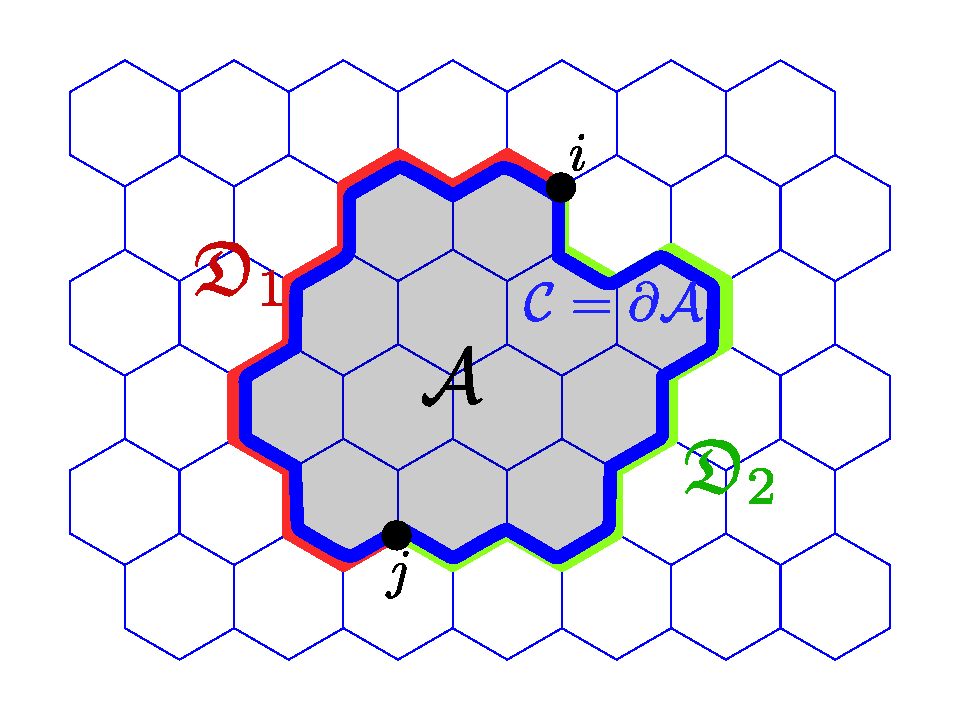
\includegraphics[width=0.45\linewidth]{figures/equivalent_loop.pdf}
    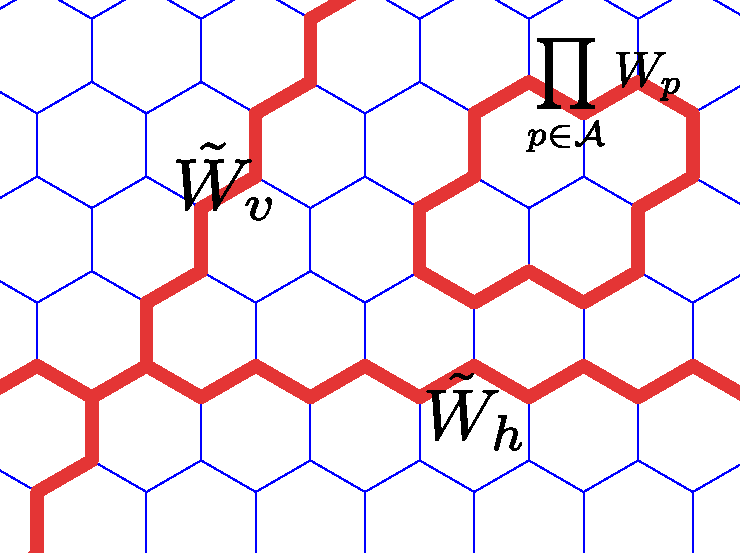
\includegraphics[width=0.45\linewidth]{figures/equivalent.pdf}
    \caption{The left panel shows two equivalent edge configurations $\mathfrak{D}_1\sim\mathfrak{D}_2$ bridged via a loop $\mathcal{C}=\de\mathcal{A}$. The two configurations share the same endpoints $i$ and $j$. The right panel shows three possible ways to get other dimer configurations with the same expectation value of the string operators. The two Wilson loops, $\Tilde{W}_h\equiv \Sigma_{\mathcal{L}_h}$ and $\Tilde{W}_v\equiv \Sigma_{\mathcal{L}_v}$ commute $[\Tilde{W}_h,\Tilde{W}_v]=0$, and neither of them can be constructed by local operators $W_p$'s. Aside from the global Wilson loops, we also have local ones, given by plaquette operators $ W_p$ inside the region $\mathcal{A}$.}
    \label{fig.equivalent}
\end{figure}
Equations~\eqref{equ.one-loop-equivalence} and \eqref{equ.string-operator-equivalent} imply an equivalence relation for edge configurations defined in such a way that two edge configurations $\mathfrak{D}_1$ and $\mathfrak{D}_2$ are \emph{equivalent}, denoted by $\mathfrak{D}_1\sim\mathfrak{D}_2$, if and only if there exists a set $\mathcal{A}$ of plaquettes such that one of the following four conditions holds:
\begin{enumerate}
    \item[(i)] $\mathfrak{D}_1=\mathfrak{D}_2\oplus\de\mathcal{A}$
    \item[(ii)] $\mathfrak{D}_1=\mathfrak{D}_2\oplus\de\mathcal{A}\oplus\mathcal{L}_v$
    \item[(iii)] $\mathfrak{D}_1=\mathfrak{D}_2\oplus\de\mathcal{A}\oplus\mathcal{L}_h$
    \item[(iv)] $\mathfrak{D}_1=\mathfrak{D}_2\oplus\de\mathcal{A}\oplus\mathcal{L}_v\oplus\mathcal{L}_h$
\end{enumerate} 
$\mathcal{L}_v$ and $\mathcal{L}_h$ are the global loop that circles the torus in the vertical and horizontal directions, the corresponding string operators of which are $\Tilde{W}_v\equiv\Sigma_{\mathcal{L}_v}$ and $\Tilde{W}_h\equiv\Sigma_{\mathcal{L}_h}$, respectively, as illustrated in the right panel of \autoref{fig.equivalent}. Equivalent configurations are collected into \emph{equivalence classes} $[\mathfrak{D}^c]=\lrg{\mathfrak{D}:\mathfrak{D}\sim\mathfrak{D}^c}$ characterized by each character $\mathfrak{D}^c$. The right panel of Fig.~\ref{fig.equivalent} shows that the two equivalent edge configurations must share the same set of endpoints, giving a simple way to identify equivalent edge configurations. In other words, there is a one-to-one correspondence between an equivalence class for edge configurations $[\mathfrak{D}]$ and the \textit{set of endpoints} of the character configuration $\mathfrak{D}$, denoted by $\mrm{EP}\lr{\mathfrak{D}}$. 
\begin{figure}
    \centering
    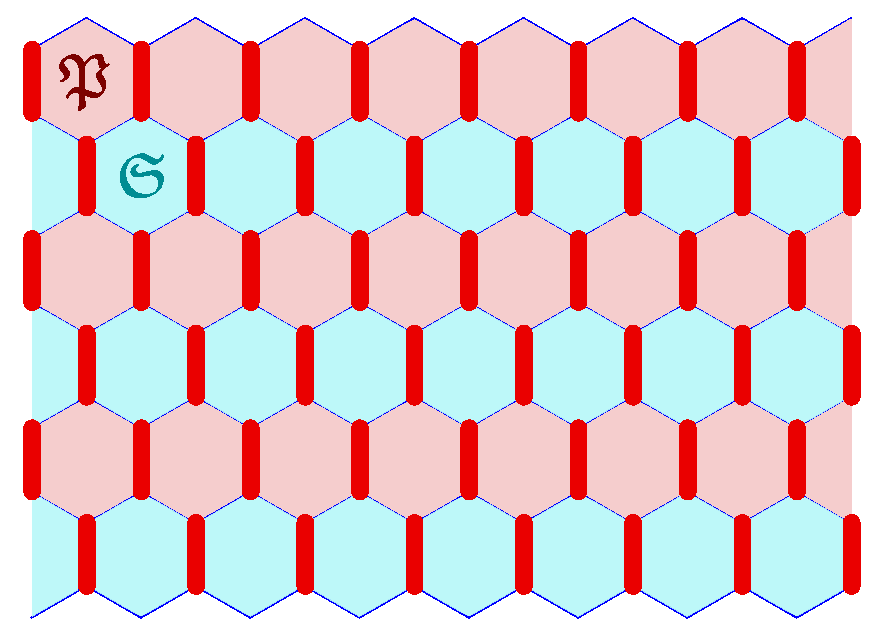
\includegraphics[width=0.48\linewidth]{figures/S-P-dimer-gas.pdf}
    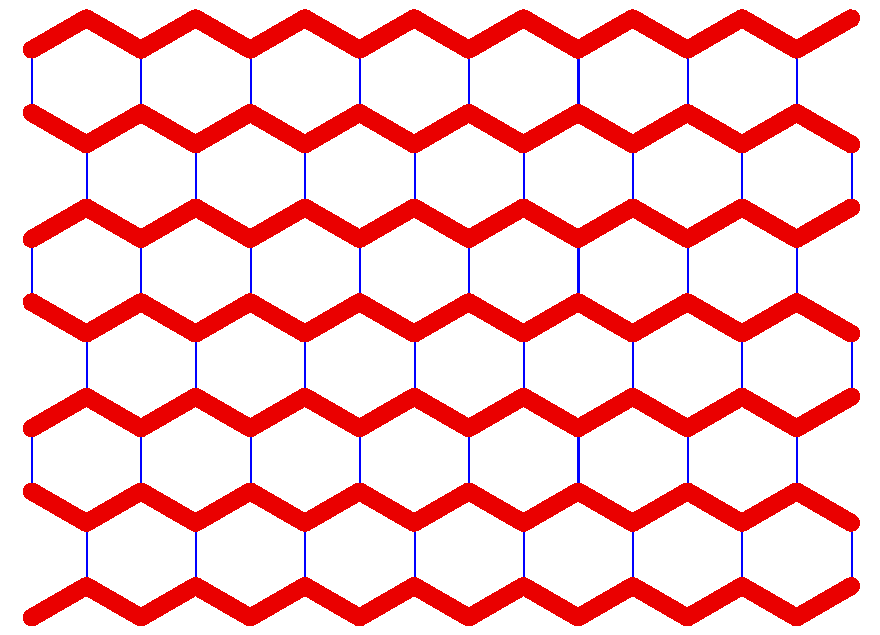
\includegraphics[width=0.48\linewidth]{figures/snake-and-dimer-gas.pdf}
    \caption{The left panel illustrates the plaqeutte configurations $\mathfrak{P}$ and $\mathfrak{S}$ as well as the edge configuration $\mathfrak{D}_Z$. The set of plaquettes in pink is denoted by $\mathfrak{P}$, while the set containing those in pink-blue is denoted by $\mathfrak{S}$. The edge configuration $\mathfrak{D}_Z$ consists of all of the red $z$-directional edges in the system, as shown in the above figure. The right panel illustrates the zigzag configuration $\mathfrak{D}_{zz}$ consisting of edges at all the horizontal loops. Such an edge configuration is also the boundary of both $\mathfrak{P}$ and $\mathfrak{S}$, for which we can write $\mathfrak{D}_{zz} = \de\mathfrak{P} = \de\mathfrak{S}$. Note that $\Sigma_{\mathfrak{D}_Z}=\Sigma_{\mathfrak{D}_{zz}}$ although $\mrm{EP}(\mathfrak{D}_Z)\neq \mrm{EP}(\mathfrak{D}_{zz})=\varnothing$} 
    \label{fig.S-P-dimer-gas}
\end{figure}

String operators of edge configurations in the same class have the same magnitude of expectation values,
\[
\abs{\anglelr{\Sigma_{\mathfrak{D}}}} = \abs{\anglelr{\Sigma_{\mathfrak{D}'}}} \quad\text{if $\mathfrak{D}\sim\mathfrak{D}'$}
\]
hence contribute the same weight to the density matrix. Nevertheless, it is still possible for two configurations from different classes to have the same weight contribution to the density matrix. There are a type of plaquette configurations, $\mathfrak{P}$ and $\mathfrak{S}$, that transform an edge configuration $\mathfrak{D}$ to $\mathfrak{D}\oplus\mathfrak{D}_Z$ because of the following relation
\begin{equation}\label{equ.P-S-dimer}
    \prod_{p\in\mathfrak{P}}W_p = \prod_{p\in\mathfrak{S}}W_p = \prod_{\anglelr{ij}\in \mathfrak{D}_Z}\sigma_i^z\sigma_{j}^z = \Sigma_{\mathfrak{D}_Z}.
\end{equation}
The plaquette configurations $\mathfrak{P}$ and $\mathfrak{S}$ as well as the edge configuration $\mathfrak{D}_Z$ are illustrated in the left panel of \autoref{fig.S-P-dimer-gas}. The edge configuration $\mathfrak{D}_Z$ is composed of the $z$-directional dimers all over the system. The plaquette configuration $\mathfrak{P}$ contains all the plaquettes at the even horizontal layers, while $\mathfrak{S}$ is the complement of $\mathfrak{P}$. The endpoint configuration $\mrm{EP}(\mathfrak{D}_Z)$ is simply the set of all the lattice sites in the system. On the other hand, the operators $\prod_{p\in\mathfrak{P}}W_p$ and $\prod_{p\in \mathfrak{S}}W_p$ is also equal to the string operator of the zigzag edge configuration $\mathfrak{D}_{zz}$, a set of all the $x$- and $y$-edges, as illustrated in the right panel of \autoref{fig.S-P-dimer-gas}
\begin{equation}\label{equ.M-MZ-complement}
\prod_{p\in\mathfrak{P}}W_p = \prod_{p\in\mathfrak{S}}W_p  = \Sigma_{\mathfrak{D}_{zz}}
\end{equation}
because $\de\mathfrak{P} = \de\mathfrak{S} = \mathfrak{D}_{zz}$.  Unlike $\mathfrak{D}_Z$, this edge configuration has no endpoints, $\mrm{EP}(\mathfrak{D}_{zz})=\varnothing$, and is equivalent to vacuum. So, we need to keep in mind that every two configurations, $\mathfrak{D}\oplus\mathfrak{D}_Z$ and $\mathfrak{D}\oplus\mathfrak{D}_{zz}$, give an identical string operator, although they are not equivalent.

We would also like to show that the physical meaning of the operator $\Sigma_{\mathfrak{D}_Z}$ is exactly the total fermion parity of the $c$-Majorana fermions. Because the expectation values of fluxes are fixed to be $\anglelr{W_p}=+1$ in the ground state, we directly know that the expectation value of $\Sigma_{\mathfrak{D}_Z}$ is equal to $+1$ directly from equation \eqref{equ.P-S-dimer} 
\begin{equation}\label{equ.fermion-parity-dimer-rep}
    \anglelr{\Sigma_{\mathfrak{D}_Z}}=1
\end{equation}
It is also worth mentioning that the combination of the plaquette operator over $\mathfrak{P}$ and the string operators containing $z$-dimers all over the lattice is equal to multiplying all edges in the entire lattice $\Lambda$ together
\begin{equation}\label{equ.fermion-parity-spin-rep}
    \lr{\prod_{p\in\mathfrak{P}}W_p} \Sigma_{\mathfrak{D}_Z} = \prod_{\anglelr{ij}\in\Lambda}\dimer{i}{j} = \mathds{1}
\end{equation}
This is nothing but the identity operator of the entire system because of the geometry of the honeycomb lattice. We can understand equations \eqref{equ.fermion-parity-dimer-rep} and \eqref{equ.fermion-parity-spin-rep} in the sense of fermion parity. In our convention, the gauge is fixed as $u_{ij}=1\forall\anglelr{ij}$, therefore, the string operator corresponding to the edge configuration that contains all of the edges in the lattice, as appeared in the last equation, transforms into the fermion parity operator $\hat{\bog{\pi}}$ up to a phase~\footnote{Two distinct Majorana fermions, say $c_1$ and $c_2$, can combine to form a normal fermion degree of freedom $f$ in a way that $f=\frac{1}{2}\lr{c_1+ic_2}$ and $f^\dagger=\frac{1}{2}\lr{c_1-ic_2}$. In this way, the fermion parity operator represented using the Majorana fermions becomes $\hat{\bog{\pi}}\equiv(-1)^{f^\dagger f}=ic_1c_2$. In a more general sense, the fermion parity operator is equal to the multiplication of all the Majorana fermions $\prod_i c_i$ up to a phase.}
\begin{equation}\label{equ.total-fermion-parity-entire-system}
    \prod_{\anglelr{ij}\in\Lambda}\dimer{i}{j}\to \prod_{\anglelr{ij}\in \Lambda}ic_ic_j
\propto \prod_{i\in\Lambda}c_i\propto \hat{\bog{\pi}}
\end{equation}
This is also due to the geometric feature of the honeycomb lattice, in which three connected edges share a lattice site. Similarly, the operator $\Sigma_{\mathfrak{D}_Z}$ in the Majorana representation is also equal to the fermion parity operator
\begin{equation}\label{equ.total-fermion-parity-Sigma-Z}
    \Sigma_{\mathfrak{D}_Z} \to \prod_{\anglelr{ij}\in\mathfrak{D}_Z}ic_ic_j\propto \prod_{i\in\Lambda}c_i\propto\hat{\bog{\pi}},
\end{equation}
because, as we will emphasize later, Majorana fermions emerge at the endpoints of each $z$-directional dimer, thus $\mrm{EP}(\mathfrak{D}_Z)$ is exactly the whole lattice system $\Lambda$. From the Majorana fermion point of view, the fermionic representation of the Kitaev Hamiltonian \eqref{equ.MF-Hamiltonian} is quadratic. As a consequence, the total fermion parity of the whole system should be conserved and must be $+1$ on a torus~\cite{Fu-Knolle-Perkins-2018}. This fermion parity degree of freedom is emergent only in the Majorana representation, and should be fixed by the intrinsic property of the spin operators in the physical spin representation. This is why the expectation value of the operator $\Sigma_{\mathfrak{D}_Z}$ is $+1$. 

Aside from the convenience arising from the fact that endpoint-point sets uniquely determine the equivalent class, the physical picture about the equivalence classes and endpoint sets also implies that a Pauli string in the spin representation is identical to the two Majorana fermions residing on the endpoints of the string. This can be seen in the \textit{commutation} among the endpoints of strings~\cite{Kitaev, fermion-and-string}. More details will be discussed in Section \ref{sec:Emergent-Fermions-at-the-Endpoints}. 

\subsection{Density Matrix of the Kitaev Ground State on a Torus}\label{sec:density-matrix-calculate}

So far, we have known two crucial points for constructing the density matrix. The first one is that finite spin-correlation functions of the Kitaev ground state must be of the following form
\[
\anglelr{\prod_{\anglelr{ij}\in \mathfrak{D}}\sigma^{\alpha_{ij}}_i\sigma^{\alpha_{ij}}_j} = \anglelr{\Sigma_{\mathfrak{D}}} \equiv \mathfrak{C}_{\mathfrak{D}}
\]
Otherwise, the correlation function vanishes. From now on, we denote by $\mathfrak{C}_{\mathfrak{D}}$ the expectation values of the string operator corresponding to the edge configuration $\mathfrak{D}$. The other is that every edge configuration in the same equivalence class gives the same weight to the density matrix, so we can sort terms in the expansion \eqref{equ.rho-starting} into equivalence classes
\begin{equation}\label{equ.class-sum}
    \sum_{\mathfrak{D}}\mathfrak{C}_{\mathfrak{D}}\Sigma_\mathfrak{D} = \sum_{[\mathfrak{D}^c]}\sum_{\mathfrak{D}\in[\mathfrak{D}^c]}\mathfrak{C}_{\mathfrak{D}}\Sigma_\mathfrak{D}
\end{equation}
From \eqref{equ.string-operator-equivalent}, we also know that every term of \eqref{equ.class-sum} in an equivalence class can be related to each other via the projector $\mathcal{P}^{(p)}$. Altogether, applying a projector $\mathcal{P}^{(p)}$ is exactly factorizing the density matrix into groups that include every edge configuration in an equivalence class $\sum_{\mathfrak{D}\in [\mathfrak{D}^c]}$, and the form of the density matrix should contain only characters of different classes $[\mathfrak{D}^c]$. Therefore, we anticipate that the form of the density matrix is of the following form
\begin{equation}\label{equ.rho-factorization}
    \rho = C \mathcal{P}_{\mrm{topo}} \sum_{[\mathfrak{D}]} \mathcal{P}^{(p)} \mathfrak{C}_{\mathfrak{D}} \Sigma_{\mathfrak{D}}
\end{equation}
where the topological Wilson-loop projector 
\[
\mathcal{P}_{\mrm{topo}}\equiv \lr{\frac{\mathds{1}+\Tilde{W}_h}{2}}\lr{\frac{\mathds{1}+\Tilde{W}_v}{2}}
\]
is imposed to include configurations related by global loops $\mathcal{L}_v$ and $\mathcal{L}_h$ illustrated in \autoref{fig.equivalent}. The constant $C$ is the normalization factor, which will be determined by imposing the constraint $\Tr\rho = 1$. Carrying out the trace 

\begin{align}\label{equ.rho-direct-trace-1}
    \Tr\rho &= \frac{C}{4} \sum_{[\mathfrak{D}]} \mathfrak{C}_{\mathfrak{D}} \Tr\lr{\mathcal{P}^{(p)}\Sigma_{\mathfrak{D}}} \nonumber\\
    &= \frac{C}{2^{2+N_p}} \sum_{[\mathfrak{D}]} \sum_{\mathcal{A}}'\Tr\lrm{ \lr{2\prod_{p\in\mathcal{A}} W_p}\Sigma_{\mathfrak{D}}}
\end{align}
The coefficient $1/4$ in the first line originates from the denominator of $\mathcal{P}_{\mrm{topo}}$. The two global Wilson-loop operators drop out because neither the local plaquette operators nor the string operators can annihilate them to yield the identity; consequently, their contributions vanish upon taking the trace. The summation of plaquette operators arises from the expansion of $\mathcal{P}^{(p)}$
\begin{align}\label{equ.W-prod-expansion}
    \prod_{p}\lr{\mathds{1}+W_p} &= \lr{\mathds{1}+\prod_{p}W_p}\sum'_{\mathcal{A}}\prod_{p\in\mathcal{A}}W_p \nonumber\\
    &= 2\sum'_{\mathcal{A}}\prod_{p\in\mathcal{A}}W_p.
\end{align}
with $\mathcal{A}$ denoting different sets of plaqette configurations defined in \eqref{equ.lattice-Stokes}. We point out that, due to the identity $\prod_{p}W_p=\mathds{1}$, the loop constructed by $\prod_{p\in \mathcal{A}}W_p$ is identical to that constructed by $\prod_{p\in \overline{\mathcal{A}}}W_p$ with $\overline{\mathcal{A}}$ representing the complement of $\mathcal{A}$. Therefore, we only need to sum over distinct loops, and the sum with a prime symbol on top in \eqref{equ.W-prod-expansion} precisely stands for such a summation. The only two terms that contribute to the trace in \eqref{equ.rho-direct-trace-1} are (i) $\mathcal{A}=\varnothing$ and $\mathfrak{D}\sim \varnothing$ and (ii) $\mathcal{A}=\mathfrak{P}$ and $\mathfrak{D}\sim\mathfrak{D}_Z$. Therefore, \eqref{equ.rho-direct-trace-1} is equal to 
\[
\Tr\rho = \frac{C}{2^{N_p}}\Tr\mathds{1} = \frac{C}{2^{-N+N_p}}
\]
To make the trace equal to $1$, we require $C = 2^{-N+N_p}$. In the end, we obtain the exact form of the density matrix
\begin{equation}\label{equ.density-matrix}
    \rho =  \frac{1}{2^{N-N_p}}\mathcal{P}_{\mrm{topo}}\mathcal{P}^{(p)}\sum_{[\mathfrak{D}]}\mathfrak{C}_{\mathfrak{D}}\Sigma_{\mathfrak{D}}
\end{equation}
Because $[W_p,\Sigma_\mathfrak{D}]=0\;\forall p,\mathfrak{D}$, the projectors $\mathcal{P}^{(p)}$ and $\mathcal{P}_{\mrm{topo}}$ commute with the summation part consisting of string operators. This is also a manifestation of the separability of the $c$-Majorana fermion sector from the gauge sector, which will be elucidated in later sections.

\subsection{Emergent Fermions at the Endpoints of Strings -- Equivalence between Spin and Fermion Representation}\label{sec:Emergent-Fermions-at-the-Endpoints}
In Appendix \ref{appendix:Majorana-derivation}, we will give another way of deriving the ground state density matrix of the Kitaev model, which starts from the Majorana representation. We will see in equation \eqref{equ.Majorana-density-matrix} that the ground state density matrix can also be represented as
\[
  \rho = 2^{N-1}\mathcal{P}_G\prod_{\anglelr{ij}}\lr{\frac{\mathds{1}+\hat{u}_{ij}}{2}}\rho_F\mathcal{P}_G
\]
where $\rho_F$ is the density matrix of the Kitaev ground state in the Majorana fermion representation and $\mathcal{P}_G$ is the Gutzwiller projection \cite{burnell-nayak, projector-1, projector-2}. The Majorana density matrix $\rho_F$ can be constructed from a starting point similar to equation \eqref{equ.rho-starting} we have used at the very beginning
\begin{equation}\label{equ.rho-F}
    \rho^F = \frac{1}{2^{N/2}}\sum_{[\mathfrak{D}]}\mathfrak{C}_\mathfrak{D}\mathcal{M}_\mathfrak{D}
\end{equation}
where
\begin{equation}\label{equ.V-rep-def}
    \mathcal{M}_\mathfrak{D} \equiv \prod_{\anglelr{ij}\in\mathfrak{D}}ic_jc_i
\end{equation}
In each dimer $\anglelr{ij}$ of the above product, the site $i$ belongs to sublattice $A$ and $j$ to sublattice $B$. The denominator of the normalization coefficient is $2^{N/2}$ instead of $2^N$ because a normal fermion $f$ is defined by two $c$-Majorana fermions $c_1$ and $c_2$ as $f=\frac{1}{2}(c_1+ic_2)$ and $f^\dagger=\frac{1}{2}(c_1-ic_2)$. Therefore, the total number of physical degrees of freedom of a system composed of $N$ Majorana fermions is $2^{N/2}$ instead of $2^N$. To manifest the similarity between the spin density matrix \eqref{equ.density-matrix}, we define a set of operators $\mathcal{S}_{\mathfrak{D}}$ for each operator that corresponds to an edge configuration
\begin{equation}\label{equ.S-def}
    \mathcal{S}_\mathfrak{D} \equiv \mathcal{P}_{\mrm{topo}}\mathcal{P}^{(p)}\Sigma_\mathfrak{D}
\end{equation}
Given equation \eqref{equ.Sigma-representation} and the fact that $[\mathcal{P}_G,\Sigma_{\mathfrak{D}}]=0$, the set of operators $\lrg{\mathcal{S}_{\mathfrak{D}}}$ also forms a representation of the algebra of edge configurations $\anglelr{\lrg{\mathfrak{D}},\oplus}$, 
\begin{equation}\label{equ.U-rep-algebra}
    \mathcal{S}_{\mathfrak{D}}\mathcal{S}_{\mathfrak{D}'} = g(\mathfrak{D},\mathfrak{D}')\mathcal{S}_{\mathfrak{D}\oplus\mathfrak{D}'}.
\end{equation}
With the string representation \eqref{equ.S-def} and \eqref{equ.U-rep-algebra}, The form of the density matrix in Eq.~\eqref{equ.density-matrix} becomes
\begin{equation}\label{equ.rho-U}
    \rho =  \frac{1}{2^{N-N_p}} \sum_{[\mathfrak{D}]}\mathfrak{C}_{\mathfrak{D}}\mathcal{S}_{\mathfrak{D}}
\end{equation}
which is of a form extremely similar to \eqref{equ.rho-F} if those $\mathcal{S}$-operators are replaced by $\mathcal{M}$-operators. This is reminiscent of different representations of the same algebra.
If we use the Majorana fermions to represent spin operators as $\sigma^\mu\to ib^\mu c$, then 
\begin{align*}
    \mathcal{S}_\mathfrak{D} &\to \mathcal{P}^{(p)} \prod_{\anglelr{ij}\in \mathfrak{D}}\lr{\hat{u}_{ij}ic_jc_i} \\
    &= \mathcal{P}^{(p)} \lrm{\prod_{\anglelr{ij}\in \mathfrak{D}}\hat{u}_{ij}} \mathcal{M}_{\mathfrak{D}}
\end{align*}
The first two products completely consist of $\hat{u}_{ij}$'s, which commute with each other as well as the $c$-Majorana fermion operators~\footnote{Note that the projector $\mathcal{P}^{(p)}$ becomes
\[\mathcal{P}^{(p)} \to \prod_{ p}\lr{\frac{\mathds{1} + \prod_{\anglelr{ij}\in p}\hat{u}_{ij}}{2}}\]
in the Majorana representation, where ``$\anglelr{ij}\in p$'' stands for \textit{those edges of the plaquette $p$}.}. Therefore, they will not contribute to the phase factor $g\lr{\mathfrak{D},\mathfrak{D}'}$ at all. So, we know that the anti-commutation relations among $c$-Majorana fermions are encoded in the phase factor $g\lr{\mathfrak{D},\mathfrak{D}'}$. In view of this, we find that the set of operators $\mathcal{M}_\mathfrak{D}$ defined by equation \eqref{equ.V-rep-def} also forms a projective representation of the edge configuration algebra and shares the same phase factor $g\lr{\mathfrak{D},\mathfrak{D}'}$ with the representation $\mathcal{S}$
\begin{equation}\label{equ.V-rep-algebra}
    \mathcal{M}_{\mathfrak{D}}\mathcal{M}_{\mathfrak{D}'} = g(\mathfrak{D},\mathfrak{D}')\mathcal{M}_{\mathfrak{D}\oplus\mathfrak{D}'}
\end{equation}
This clearly illustrated a picture: the Majorana fermion representation is identical to the spin, or Pauli string, representation, and the Majorana fermions can be seen as emerging from the endpoints of those Pauli strings defined by \eqref{equ.string-operator-def}~\cite{Kitaev, fermion-and-string, string-net, Photons-and-electrons-as-emergent-phenomena-string, PRD-string-wen-quantum-order}. Remember that the core principle that allows us to describe the Kitaev model using gauge theory is the fractionalization of spin degrees of freedom into Majorana fermions and gauge fields. To analyze everything in spin language, we have to always represent everything in strings in such a way that two Majorana fermions or gauge field operators in every pair, which appear in the gauge theory after the fractionalization of the spin degrees of freedom, are connected by a string. More vividly speaking, we have to \textit{glue} those fractionalized degrees of freedom back via string operators defined in spin language. From this perspective, the fermion anticommutation relation is clearly evident in \autoref{fig.standard-configuration}. 
\begin{figure}
    \centering
    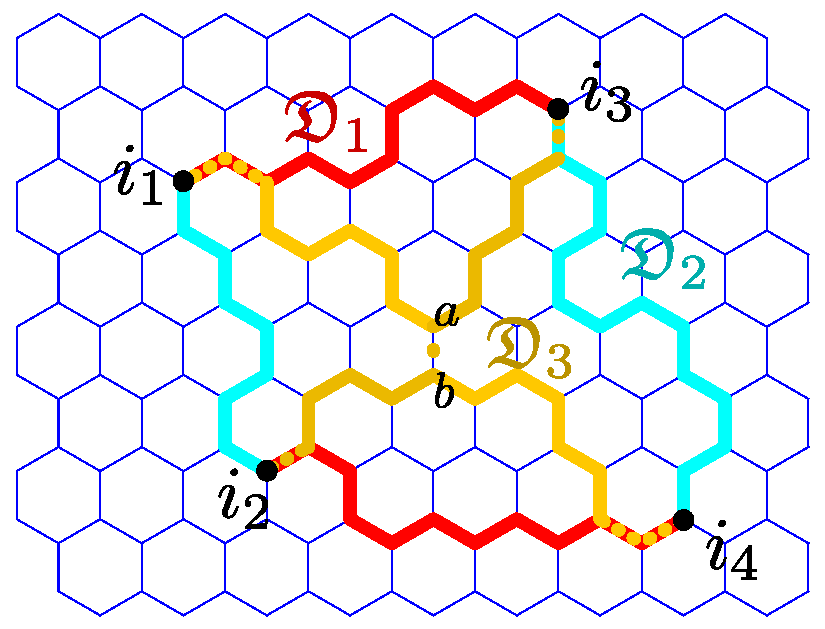
\includegraphics[width=0.7\linewidth]{figures/exchange.pdf}
    \caption{$\mathfrak{D}_1$ and $\mathfrak{D}_2$ are equivalent configurations because they share the same set of endpoints. $\mathfrak{D}_2$ can be decomposed into two strings ($\overline{i_1i_2}$ and $\overline{i_3i_4}$) that connect different types of endpoints, while $\mathfrak{D}_1$ is composed of two strings ($\overline{i_1i_3}$ and $\overline{i_2i_4}$) connecting the same type of endpoints. Another configuration $\mathfrak{D}_3$ is the combination of two strings ($\overline{i_1i_4}$ and $\overline{i_2i_3}$) connecting different types of endpoints. Still, the intersection part (brown dotted segment $\overline{ab}$ at the center of the figure) vanishes because the combination is accomplished by performing $\oplus$ between the two edge configurations, making it equivalent to the combination of two strings $\overline{i_1i_3}$ and $\overline{i_2i_4}$ with the order of $i_3$ and $i_4$ being swapped. }
    \label{fig.standard-configuration}
\end{figure}
In the illustration, there are three different ways, $\mathfrak{D}_1$, $\mathfrak{D}_2$, and $\mathfrak{D}_3$, to connect four points, $i_1$, $i_2$, $i_3$, and $i_4$. The expectation values of the first two configurations are the same, only with a sign difference. Mathematically, it can be expressed as $\mathcal{S}_{\overrightarrow{i_1i_2}}\mathcal{S}_{\overrightarrow{i_3i_4}} = -\mathcal{S}_{\overrightarrow{i_1i_3}}\mathcal{S}_{\overrightarrow{i_2i_4}}$. The subscript $\overrightarrow{ij}$ not only indicates a string configuration $\overline{ij}$ illustrated in \autoref{fig.standard-configuration} but also specifies the ordering of the product in \eqref{equ.string-operator-def}. This relation can be verified directly by considering the commutation relations among spin operators and the fact that the combination of the two configurations $\mathfrak{D}_1\oplus \mathfrak{D}_2 \sim \varnothing$ is a closed loop. If we treat the four endpoints of strings as the position of fermions, then the sign flipping can be understood as a consequence of exchanging the arrangement of the fermion operator from $\lr{c_{i_1}c_{i_2}}\lr{c_{i_3}c_{i_4}}$ to $\lr{c_{i_1}c_{i_3}}\lr{c_{i_2}c_{i_4}}$. The third configuration $\mathfrak{D}_3$ can be shown to be identical to $\mathfrak{D}_1$ because the intersection $\overline{ab}$ of the two segments $\overline{i_1i_4}$ and $\overline{i_2i_3}$ is equivalent to vacuum after taking the symmetric difference $\oplus$. The flip of the sign is also crucial here despite the equivalence between the two configurations. This is due to the anticommutation relation among three connected dimers,
\[
\segment{i}{,i+\mu}\segment{i}{,i+\mu'} = (-1)^{\delta_{\mu,\mu'}+1}\segment{i}{,i+\mu'}\segment{i}{,i+\mu}
\]
where $\mu,\mu'=x,y,z$ indicates the direction of the dimers. With this relation, a flip of the sign arising from a swap of $i_3$ and $i_4$ can be shown directly in the following,
\begin{align*}
    \segment{i_1}{i_4}\segment{i_2}{i_3} &= \segment{i_1}{a}\segment{a}{b}\segment{b}{i_4} \segment{i_2}{b}\segment{b}{a}\segment{a}{i_3} \\
    &= -\segment{i_1}{a}\segment{a}{i_3} \segment{i_2}{b}\segment{b}{i_4} \segment{a}{b}\segment{b}{a} 
    = -\segment{i_1}{i_3}\segment{i_2}{i_4}.
\end{align*}
This result is in agreement with the relation $(c_{i_1}c_{i_4})(c_{i_2}c_{i_3}) = -(c_{i_1}c_{i_3})(c_{i_2}c_{i_4})$.
\begin{figure}
    \centering
    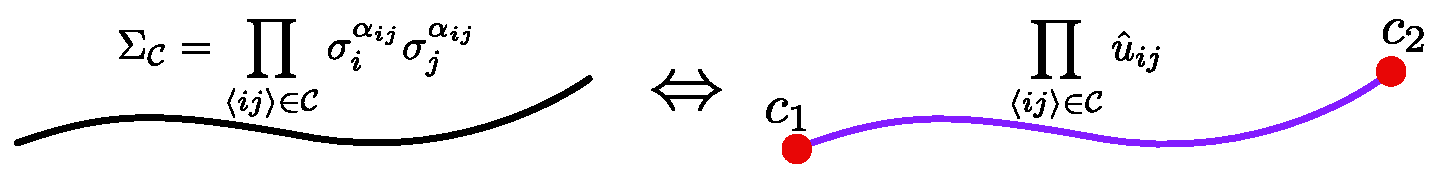
\includegraphics[width=\linewidth]{figures/linking-string.pdf}
    \caption{Two Majorana fermions emerge at the endpoints of a string $\mathcal{C}$. In the fermion representation, the link that connects the two $c$-Majorana fermions is composed of $\mathbb{Z}_2$ gauge-field operators, $\prod_{\anglelr{ij}\in\mathcal{C}} \hat{u}_{ij}$.}
    \label{fig.linking-strings}
\end{figure}

In conclusion, it has been demonstrated that the $\mathcal{M}$-representation is identical to the $\mathcal{S}$-representation. This phenomenon can be understood as follows. Two Majorana fermions, $c_1$ and $c_2$, connected by a string $\mathcal{C}$ of $\mathbb{Z}_2$ gauge-field operators, generate a string operator~\cite{Kitaev}, as illustrated in \autoref{fig.linking-strings}
\[
c_1\lr{\prod_{\anglelr{ij}\in\mathcal{C}} \hat{u}_{ij}}c_2 = \prod_{\anglelr{ij}\in\mathcal{C}}c_i\hat{u}_{ij}c_j \propto \prod_{\anglelr{ij}\in\mathcal{C}}\dimer{i}{j} = \Sigma_{\mathcal{C}}
\]
up to a phase depending on the length of the string $\mathcal{C}$. This relation clearly illustrates that the $c$-Majorana fermions emerge at the endpoints of strings.

\subsection{Reduced Density Matrix}\label{sec:density-matrix-reduced}
Information about many-body entanglement of a state is encoded in reduced density matrices $\rho_A$, which implies the entanglement properties between the subregion $A$ and its environment $\overline{A}$, i.e., the rest of the system. In the previous sections, we have rigorously obtained the exact form of the density matrix of the Kitaev ground state. We further find that it is straightforward to get the reduced density matrix $\rho_A$ by tracing out the environment directly $\rho_A = \Tr_{\overline{A}}\rho$. Despite the rigorous derivation of how to carry out the trace shown in Appendix~\ref{appendix:reduced-density0matrix}, there is also an intuitive way to get the reduced density matrix. Following the logic of the previous discussion, the property of a reduced density matrix is pretty much the same as the density matrix of the whole system, since both are designed to give the expectation values of observables in the way that $\anglelr{\mathcal{O}_A}=\Tr\lr{\rho\mathcal{O}_A}=\Tr_A\lr{\rho_A\mathcal{O}_A}$, for any observable $\mathcal{O}_A$ with support $A$. As we know, in the Kitaev model, observables possessing finite expectation values are string operators. Therefore, the reduced density matrix can be expressed in terms of string operators $\Sigma_\mathfrak{D}$, with $\mathfrak{D}$ entirely inside $A$, accompanied by their expectation values $\mathfrak{C}_\mathfrak{D}$,
\begin{equation}\label{equ.rho-A-raw-guess}
    \rho_A \propto\sum_{\mathfrak{D}\subset A}\mathfrak{C}_\mathfrak{D} \Sigma_\mathfrak{D}
\end{equation}
After that, the equivalent configurations can be sorted in the same way as in the previous section, then the summation can be rewritten as a summing of equivalent classes with the projector $\mathcal{P}^{(p)}_A$ of dimension $2^{N^A-N^A_p}$, which only includes plaquettes inside $A$,
\begin{equation}\label{equ.p-proj-A}
    \mathcal{P}^{(p)}_A = \prod_{p\in A}\lr{\frac{\mathds{1}+W_p}{2}}
\end{equation}
The final form of the reduced density matrix is then
\[
\rho_A = C\mathcal{P}^{(p)}_A\sum_{[\mathfrak{D}]\subset A}\mathfrak{C}_{\mathfrak{D}}\Sigma_{\mathfrak{D}}
\]
The condition $[\mathfrak{D}]\subset A$ below the summation means choosing equivalence classes such that each class contains at least one configuration that is entirely contained within $A$. Recall the correspondence between endpoint sets and equivalent classes, the condition is also equivalent to choosing classes $[\mathfrak{D}]$ such that $\mrm{EP}(\mathfrak{D})\subset A$. The constant $C$ is a normalization coefficient to be determined by imposing the normalization condition $\Tr_A\rho_A=1$,
\begin{align*}
    \Tr_A\rho_A &= C\sum_{[\mathfrak{D}]\subset A} \mathfrak{C}_\mathfrak{D} \Tr_A\lrm{\mathcal{P}^{(p)}_A \Sigma_\mathfrak{D}} \\
    &= \frac{C}{2^{N^A_p}}\sum_{\mathcal{A}_p}\sum_{[\mathfrak{D}]\subset A} \mathfrak{C}_\mathfrak{D} \Tr_A\lrm{ \lr{\prod_{p\in\mathcal{A}_p}W_p} \Sigma_\mathfrak{D}} \\
    &= \frac{C}{2^{N^A_p}}\Tr_A\mathds{1}_A = C2^{N^A - N^A_p} = 1
\end{align*}
Therefore, the final form of the reduced density matrix is as follows.
\begin{equation}\label{equ.red-den-mat-sim-con}
    \rho_A = \frac{1}{2^{N^A-N^A_p}} \mathcal{P}^{(p)}_A\sum_{[\mathfrak{D}]\subset A}\mathfrak{C}_{\mathfrak{D}}\Sigma_{\mathfrak{D}}
\end{equation}
The form \eqref{equ.red-den-mat-sim-con} is the same as the density matrix \eqref{equ.density-matrix} as we anticipated. Along a similar line, we can also define a set of $\mathcal{S}$-operators
\begin{equation}\label{equ.U-A-def}
    \mathcal{S}^{(A)}_\mathfrak{D} \equiv \mathcal{P}^{(A)}\Sigma_\mathfrak{D}
\end{equation}
supported on the subregion $A$. With these newly defined operators, the reduced density matrix becomes
\begin{equation}\label{equ.red-DM-new}
    \rho_A = \frac{1}{2^{N^A-N^A_p}}\sum_{[\mathfrak{D}]\subset A}\mathfrak{C}_{\mathfrak{D}}\mathcal{S}^{(A)}_\mathfrak{D}.
\end{equation}
The form of the reduced density matrix above implies that the physical picture of Majorana fermions emerging at the endpoints of string operators still holds in any simply-connected subregion $A$, and it can be verified that $\mathcal{S}^{(A)}$-operators also satisfy a relation
\begin{equation}\label{equ.U-A-rep-algebra}
    \mathcal{S}^{(A)}_{\mathfrak{D}}\mathcal{S}^{(A)}_{\mathfrak{D}'} = g(\mathfrak{D},\mathfrak{D}')\mathcal{S}^{(A)}_{\mathfrak{D}\oplus\mathfrak{D}'},
\end{equation}
which is the same as \eqref{equ.U-rep-algebra} and \eqref{equ.V-rep-algebra}. The reduced density matrix of Majorana fermions in the region $A$ also possesses the same form 
\begin{equation}\label{equ.rho-F-reduced}
    \rho_A^{F} \equiv \frac{1}{2^{N^A/2}}\sum_{[\mathfrak{D}]\subset A}\mathfrak{C}_{\mathfrak{D}}\mathcal{M}_\mathfrak{D}
\end{equation}
There are two straightforward ways to obtain this conclusion. The first approach is to trace out the environment of the Majorana fermion density matrix \eqref{equ.rho-F}. Because every $\mathcal{M}_\mathfrak{D}$ is a $\mathbb{Z}_2$ operator and thus $\Tr \mathcal{M}_{\mathfrak{D}}=0$ if $\mathfrak{D}\not\sim\varnothing$, the remaining part therefore consists of terms with $[\mathfrak{D}]\subset A$, which constitutes the reduced density matrix of a simply-connected region $A$.  The second way is following the logic of \eqref{equ.rho-A-raw-guess}. The observables in the Majorana space with finite expectation values are exactly $\mathcal{M}_\mathfrak{D}$ operators. To ensure that the reduced density matrix $\rho^F_A$ preserves the correct expectation values for these operators, the form of $\rho^F_A$ must be of \eqref{equ.rho-F-reduced}. Here, we only consider regions with an even $N^A$ since the denominator $2^{N^A/2}$ becomes fractional if $N^A$ is an odd number, making the dimension of the Hilbert space ill-defined. In the latter sections, cases with an odd number of $N^A$ will be discussed. 

\section{Entanglement Properties}
So far, we have thoroughly discussed the density matrices of the Kitaev ground state in various situations. Here, based on the density matrices we found in previous sections, we investigate the structure of the entanglement spectrum of the Kitaev model. In this study, we will still represent the final result of the entanglement spectra of the Kitaev model in terms of the entanglement spectra of the free Majorana fermion systems, as proposed in Ref.~\cite{Yao-Qi}. On the one hand, it is not feasible to directly analyze the entanglement spectra using spin language because of the complex algebraic features of spin operators; On the other hand, the degeneracy in the entanglement spectrum and the block-diagonal feature of the reduced density matrices actually shed more physical insights into the origin of the gauge contribution to the entanglement, as the physical picture provided by Ref.~\cite{PRX-ent-high}. 

\subsection{Even Number of Sites}\label{sec:EE-calculation-even}
As we have discussed in Section~\ref{sec:Emergent-Fermions-at-the-Endpoints}, there is a clear correspondence, manifested by \eqref{equ.U-rep-algebra} and \eqref{equ.V-rep-algebra}, between operators $\mathcal{S}_\mathfrak{D}$ and $\mathcal{M}_\mathfrak{D}$. In the subregion, after tracing out the environment, a similar relation is still there between $\mathcal{S}^{(A)}_\mathfrak{D}$ and $\mathcal{M}_\mathfrak{D}$ for all $\mathfrak{D}\subset A$. Due to the equivalence of the representations $\mathcal{S}^{(A)}$ and $\mathcal{M}$ in the region $A$, plus the similarity of the forms of \eqref{equ.red-DM-new} and \eqref{equ.rho-F-reduced}, the entanglement entropy of the spin system $S_A = \Tr_A\rho_A\ln\rho_A$ can be calculated through the Majorana density matrix \eqref{equ.rho-F-reduced} as an alternative. Inspired by this insight, we first observe that both representations $\mathcal{S}^{(A)}$ and $\mathcal{M}$ consist of traceless operators and the identity. Therefore, their trace satisfies 
\begin{equation}\label{equ.U-V-trace-relation}
    \left\{
\begin{aligned}
&\Tr_{A} \mathcal{S}^{(A)}_{\mathfrak{D}} = 2^{N^A-N^A_p}\delta_{\mathfrak{D},\varnothing} \\
& \Tr_{A,F} \mathcal{M}_{\mathfrak{D}} = 2^{N^A/2}\delta_{\mathfrak{D},\varnothing}
\end{aligned}
\right.
\end{equation}
where $\Tr_{A,F}$ stands for taking the trace over the $c$-Majorana fermion space in the region $A$. Given that the two representations are identical, the following identity holds for an arbitrary analytic function $f$: 
\begin{equation}\label{equ.identity}
    \Tr_A f(\{\mathcal{S}^{(A)}\}) = \frac{1}{2^{N^A/2 - N^A_p}}\Tr_{A,F} f(\lrg{\mathcal{M}})
\end{equation}
Given this property, we can define a function
\begin{align*}
    &f(\lrg{W}) \\
    \equiv& \lrm{\frac{1}{2^{N^A-N^A_p}}\sum_{[\mathfrak{D}]\subset A}\mathfrak{C}_\mathfrak{D}W_{\mathfrak{D}}}\ln\lrm{\frac{1}{2^{N^A-N^A_p}}\sum_{[\mathfrak{D}]\subset A}\mathfrak{C}_\mathfrak{D}W_{\mathfrak{D}}}
\end{align*}
where $W$ stands for an arbitrary representation of the algebra $\anglelr{\lrg{\mathfrak{D}},\oplus}$. With this, we further define the following two functions to compute the entanglement entropy.
\[
\left\{
\begin{aligned}
&\rho^F_A\ln\rho_A^F = \frac{1}{2^{N^A/2-N^A_p}} f\lr{\lrg{\mathcal{M}}} - \lrm{\lr{\frac{N^A}{2}-N^A_p}\ln 2}\rho^F_A \\
& \rho_A\ln\rho_A = f(\{\mathcal{S}^{(A)}\})
\end{aligned}
\right.
\]
The entanglement entropy can be written in terms of the above functions, and the trace over the spin space can be converted to the trace over the $c$-Majorana space using Eq.~\eqref{equ.identity}
\begin{align*}
    S_A &= -\Tr_A f(\{\mathcal{S}^{(A)}\}) \\
    &= -\frac{1}{2^{N^A/2 - N^A_p}}\Tr_{A,F} f(\lrg{\mathcal{M}}) \\
    &= -\Tr_{A,F} \rho^F_A\ln\rho^F_A + \lr{\frac{N^A}{2}-N^A_p}\ln 2.
\end{align*}
Here we introduce a relation that bridges $N^A$, $N^A_p$, and $\abs{\de A}$ together (its proof is given in Appendix~\ref{appendix:Pick}),
\begin{equation}\label{equ.Pick_sim-con}
    \abs{\de A} = N^A - 2N^A_p + 2
\end{equation}
With this, the terms in parentheses of the last line of the above derivation can be rewritten in terms of $\abs{\de A}$, and we get 
\begin{equation}\label{equ.EE-separation}
    S_A = \underbrace{-\Tr_{A,F}\lr{\rho_A^F\ln\rho_A^F}}_{\equiv S_A^F} + \underbrace{\lr{\frac{1}{2}\abs{\de A}-1}\ln 2}_{\equiv S_A^G}
\end{equation}
This formula shows that the entanglement entropy can be separated into the fermion part $S^F_A$ and the gauge part, $S^G_A$, in agreement with the result obtained in \cite{Yao-Qi}.

Here, we summarize our discussion on the origin of the gauge part $S^G_A$ of the entanglement entropy. From our derivation, the gauge part of the entanglement entropy arises from the difference in the dimension of the physical spin Hilbert space and the Hilbert space of the Majorana fermions. The premise that allows us to make such a comparison between the spin Hilbert space and the Majorana Hilbert space is that the spin representation $\mathcal{S}$ of the Kitaev model ground state is identical to the Majorana representation $\mathcal{M}$ in a way we have introduced. If we trace back further to the origin of such an algebraic equivalence, we will find that it arises from the concept of equivalent edge configurations because the spin correlation functions corresponding to configurations in the same equivalence class are identical. Thus, the structure of the reduced density matrix can be factorized, as manifested by equation \eqref{equ.rho-factorization}. At the same time, a gauge theory is also a way to define equivalence classes, in the sense that we identify different gauge field configurations as equivalent if one can be transformed into the other via a gauge transformation. 

The Majorana fermion entanglement entropy $S^F_A$, which appears in equation \eqref{equ.EE-separation}, can be computed exactly using the method proposed by Ref.~\cite{Jin-Korepin, Vidal-Latorre-Rico-Kitaev, Latorre-Rico-Vidal, Peschel_2003, Peschel_2009, Chung_2001, Cheong_2004} because the Kitaev ground state is equivalent to a free fermion system. For a free Majorana fermion system, multi-point correlation functions can be decomposed into two-point correlation functions thanks to Wick's theorem, so the two-point correlation functions contain complete information about the state, including the entanglement. It turns out that the single-particle entanglement spectrum is exactly the eigenvalue spectrum of the correlation matrix $\Gamma^{(c)}$, which is of size $N^A\times N^A$, defined as
\begin{equation}
    [\Gamma^{(c)}]_{ij} \equiv \frac{1}{2}\anglelr{c_ic_j}\quad ;\; i,j\in A
\end{equation}
The eigenvalues of $\Gamma^{(c)}$, denoted by $\gamma_{k,\pm}$, which are also elements in the single-particle entanglement spectrum, can be expressed in pairs if $N^A$ is even~\cite{Jin-Korepin, Latorre-Rico-Vidal}
\begin{equation}\label{equ.gamma-eigenvalue}
    \gamma_{k,\pm} = \frac{1 \pm \nu_k}{2} \quad ; \; 1,2,\cdots,N^A/2
\end{equation}
A pair of eigenvalues can also be expressed in terms of a parameter $\epsilon_k$ as 
\begin{equation}\label{equ.epsilon-k}
    \gamma_{k,n_k} = \frac{\mrm{e}^{-\epsilon_k\lr{1 - 2n_k}}}{2\tanh{\epsilon_k}}
\end{equation}
with $n_k=0,1$ implying $+,-$ in expression~\eqref{equ.gamma-eigenvalue}, respectively. There are then $2^{N^A/2}$ elements in the many-body entanglement spectrum of the whole system, which are composed of these single particle values in such a way that
\begin{equation}\label{equ.many-body-entanglement-spectrum}
    \lambda_{\lrg{n}} \equiv \prod_{k=1}^{N^A/2}\gamma_{k,n_k} = \frac{1}{\mathcal{Z}} \mrm{e}^{-\sum_{k=1}^{N^A/2} \epsilon_k \lr{1-2n_k}}
    %\prod_{k=1}^{N^A/2}\frac{1 + (-1)^{n_k}\nu_k}{2}
\end{equation} 
where $\mathcal{Z}\equiv\prod_{k=1}^{N^A/2}2\tanh\epsilon_k$. By this method, the fermion entanglement spectrum can be numerically computed if the exact form of the two-point fermion correlation functions is given, which can be obtained straightforwardly by exactly solving the Hamiltonian~\eqref{equ.MF-Hamiltonian}. With the entanglement spectrum, it is straightforward to compute the entanglement entropy, 
\begin{equation}\label{equ.EE-corr-mat}
    S_A^F = -\sum_{\lrg{n}}\lambda_{\lrg{n}}\ln \lambda_{\lrg{n}} = -\tr\lr{\Gamma^{(c)}\ln\Gamma^{(c)}}
\end{equation}
The trace ``$\tr$'' is written in lowercase here to distinguish it from the trace ``$\Tr$'' over the Hilbert space of the quantum many-body system. This quantity can be computed via numerically diagonalizing the correlation matrix $\Gamma^{(c)}$. In terms of the correlation matrix, formula \eqref{equ.EE-separation} can be written as
\begin{equation}\label{equ.Yao-Qi-standard-form}
    S_A = -\tr\lr{\Gamma^{(c)} \ln \Gamma^{(c)}} + \lr{\frac{1}{2}\abs{\de A} - 1}\ln 2
\end{equation}
where the first term is identified as the fermion part $S^F_A$, while the other is the gauge part $S^G_A$.


The derivation of the entanglement entropy reveals that the fermion part $S^F_A$ reflects the equivalence of representations $\mathcal{S}_\mathfrak{D}$ and $\mathcal{M}_\mathfrak{D}$, and the gauge part $S^G_A$ arises from the difference between the spaces supporting these two identical representations. In particular, the separability of the gauge and fermion degrees of freedom relies on two crucial properties, $[W_p, W_{p'}]=0\;\forall p,p'$ and $[W_p,\Sigma_{\mathfrak{D}}]=0\; \forall p,\mathfrak{D}$. The latter guarantees the decomposition of the spin system into gauge and matter sectors controlled by $W_p$ and $\Sigma_\mathfrak{D}$, respectively, whereas the former implies the gauge has no dynamics. 

\subsection{Odd Number of Sites}\label{sec:EE-calculation-odd}
It is much more subtle to discuss the entanglement property of cases with odd $N^A$. As we have mentioned, a single normal fermion degree of freedom is formed by a combination of two Majorana fermions. Thus, a well-defined dimension of a Hilbert space of a system composed of $c$-Majorana fermions relies on the requirement that $N^A$ must be even. However, in the physical spin representation, a region with an odd $N^A$ is supposed to be able to be analyzed in the same manner as we introduced in previous chapters. An alternative to resolve the issue of odd $N^A$ is to add a redundant Majorana fermion, denoted by $c_{(N^A+1)}$, to the original system, making the number of Majorana fermions $N^A+1$, which is even, so that our previous approach works again. This redundant Majorana fermion is defined in such a way that it has no interaction with any other Majorana fermion. In other words, $\sanglelr{ c_{(N^A+1)}c_i}=0\;\forall i\in A$. In this way, the dimension of the Hilbert space of $c$-Majorana fermions, including the redundant one, is $2^{(N^A+1)/2}$, and the reduced density matrix becomes
\begin{equation}\label{equ.rho-A-F-odd}
    \rho_A^{F} = \frac{1}{2^{\lr{N^A+1}/2}}\sum_{[\mathfrak{D}]\in A}\mathfrak{C}_{\mathfrak{D}}\mathcal{M}_\mathfrak{D}
\end{equation}
The redundant Majorana fermion does not enter the density matrix, and the form of $\rho^F_A$ remains the same. Only the normalization coefficient is changed. With the redundant Majorana fermion, the original correlation matrix $\Gamma^{(c)}$ must correspondingly be enlarged to $\Tilde{\Gamma}^{(c)}$ by one dimension. According to the definition of $c_{(N^A+1)}$, we get
\begin{equation}\label{equ.tilde-Gamma-corner}
    \Tilde{\Gamma}^{(c)} = 
\lr{
\begin{array}{c|c}
    \Gamma^{(c)} & 0 \\
    \hline
    0 & 1/2
\end{array}
}
\end{equation}
In the enlarged correlation matrix $\Tilde{\Gamma}^{(c)}$, the upper-left block is the original correlation matrix. The upper-right column and the lower-left row are zeros because the redundant Majorana fermion does not correlate with others. The element $1/2$ at the lower-right entry is given by the redundant Majorana fermion, $\frac{1}{2}=\frac{1}{2}\sanglelr{c_{(N^A+1)}c_{(N^A+1)}}$. 

Due to the change in the dimension of the Hilbert space of the $c$-Majorana sector, the relation \eqref{equ.U-V-trace-relation} needs to be modified to
\begin{equation}\label{equ.U-V-trace-relation-odd}
    \left\{
\begin{aligned}
&\Tr_{A} \mathcal{S}^{(A)}_{\mathfrak{D}} = 2^{N^A-N^A_p}\delta_{\mathfrak{D},\varnothing} \\
& \Tr_{A,F} \mathcal{M}_{\mathfrak{D}} = 2^{(N^A+1)/2}\delta_{\mathfrak{D},\varnothing}
\end{aligned}
\right.
\end{equation}
Carrying out the same calculation as we did in the even $N^A$ cases, we obtain a similar result to the entanglement entropy 
\begin{align}\label{equ.EE-odd-derive-1}
    S_A &= -\Tr_{A,F} \rho^F_A\ln\rho^F_A + \lr{\frac{N^A-1}{2}-N^A_p}\ln 2 \nonumber\\
    &= -\tr\lr{\Tilde{\Gamma}^{(c)}\ln \Tilde{\Gamma}^{(c)}} + \lr{\frac{1}{2}\abs{\de A} - \frac{3}{2}}\ln 2
\end{align}
where the correlation matrix in \eqref{equ.EE-corr-mat} is replaced by the enlarged one. According to \eqref{equ.tilde-Gamma-corner}, the first term of \eqref{equ.EE-odd-derive-1} can be reduced and expressed in terms of the original correlation matrix 
\begin{equation}\label{equ.EE-reduce}
    \tr\lr{\Tilde{\Gamma}^{(c)} \ln \Tilde{\Gamma}^{(c)}} = \tr\lr{\Gamma^{(c)} \ln \Gamma^{(c)}} - \frac{1}{2}\ln 2 
\end{equation}
Substituting \eqref{equ.EE-reduce} into \eqref{equ.EE-odd-derive-1}, we will see that the last term $-\frac{1}{2}\ln 2$ in \eqref{equ.EE-reduce}, arises from the corner of $\Tilde{\Gamma}^{(c)}$ caused by the redundant fermion,  cancels the term $-\frac{1}{2}\ln 2$ in \eqref{equ.EE-odd-derive-1} arising from the enlarged dimension of the $c$-Majorana fermion sector, and we ultimately obtain a result that is the same as \eqref{equ.Yao-Qi-standard-form} in cases with even $N^A$. From this derivation, we prove that the result obtained by \cite{Yao-Qi} is still correct for cases with odd $N^A$. The procedure can be understood in the following way. We first borrow dimension $2^{1/2}$ of a single Majorana fermion from the gauge sector to make the Hilbert space of the $c$-Majorana sector well-defined, and the additional term $-\frac{1}{2}\ln 2$ reflects such a borrowed dimension. Afterward, the redundant fermion forms an isolated corner in the correlation matrix $\Tilde{\Gamma}^{(c)}$, which gives the term $\frac{1}{2}\ln 2$ and then returns the dimension to the gauge sector. In the end, there is no net effect of the number of lattice sites, and the formula \eqref{equ.Yao-Qi-standard-form} holds for both even and odd cases.

As shown in \eqref{equ.gamma-eigenvalue}, the elements in the single-particle entanglement spectrum come in pairs. That is, if $\frac{1+\nu_k}{2}$ is an eigenvalue of $\Tilde{\Gamma}^{(c)}$, then such a matrix must have another eigenvalue $\frac{1-\nu_k}{2}$~\cite{Jin-Korepin}. As we have discussed, such a mode is designed in such a way that it decouples from other physical Majorana fermions, so we know the diagonal entry is exactly an eigenvalue of the correlation matrix $\Gamma^{(c)}$. Therefore, there must be another eigenvalue $\frac{1}{2}=1-\frac{1}{2}$ in the physical block of the correlation matrix. That means the many-body entanglement spectrum can be written as 
\begin{equation}\label{equ.many-body-entanglement-spectrum-odd}
\lambda_{n_1,n_2,\cdots,n_{(N^A+1)/2}} = \frac{1}{2}\prod_{k=1}^{\frac{N^A-1}{2}}\gamma_{k,n_k}
\end{equation}
The formula shows that the many-body entanglement spectrum essentially depends on only $(N^A-1)/2$ quantum numbers, although the complete labeling contains $(N^A+1)/2$ of them. In other words, there is a 2-fold degeneracy in the entanglement spectrum of the $c$-Majorana sector, and therefore we only have $2^{\frac{N^A-1}{2}}$ distinct eigenvalues. The degree of degeneracy for each distinct eigenvalue is therefore $2^{\frac{N^A+1}{2}-N^A_p}$ because the total number of eigenvalues is equal to the number of distinct eigenvalues multiplied by the number of degeneracies
\[
2^{N^A-N^A_p} = 2^{\frac{N^A-1}{2}}\times 2^{\frac{N^A+1}{2}-N^A_p}.
\]
Defining the entanglement Hamiltonian $\mathcal{H}_A$ as the exponent of the reduced density matrix $\rho_A = \mrm{e}^{-\mathcal{H}_A}/\Tr_A\lr{\mrm{e}^{-\mathcal{H}_A}}$, it is proven to be quadratic~\cite{Peschel_2003, Peschel_2009, Chung_2001, Cheong_2004} and can be diagonalized as 
\begin{equation}\label{equ.entanglement-Hamiltonian}
    \mathcal{H}_A = \sum_{k=1}^{\frac{N^A+1}{2}}\epsilon_k\lr{1 - 2a^\dagger_k a_k}
\end{equation}
This form has also been implied by~\eqref{equ.many-body-entanglement-spectrum}. The quantum number $n_k$ that appears in \eqref{equ.many-body-entanglement-spectrum} and \eqref{equ.many-body-entanglement-spectrum-odd} is exactly the expectation value of the fermion number operator $a^\dagger_k a_k$ that diagonalizes the entanglement Hamiltonian. From the relation of the quantum number $n_k$ with the fermion number operator and the form of the entanglement Hamiltonian, we can identify $\hat{\bog{\pi}}^{(A)}\equiv(-1)^{\sum_{k}n_k} = \prod_{k}\lr{1-2n_k}$ as the total fermion parity in the subregion $A$. In the fermion parity point of view, we can understand the 2-fold degeneracy in the $c$-Majorana sector as the block-diagonalization depending on the total fermion parity in $A$. As we have seen, the value of $\lambda_{\lrg{n}}$ is independent of the last fermion number $n_{(N^A+1)/2}$. At the same time, $\hat{\bog{\pi}}^{(A)}$ commutes with the entanglement Hamiltonian, hence also commutes with $\rho_A$. Therefore, the entanglement spectrum can be separated into even and odd sectors, and these two sectors actually correspond to $\lrg{n}$ with $n_{(N^A+1)/2}=0,1$, respectively. In all, $\rho_A$ with odd $N^A$ is block-diagonalized to two blocks, one corresponding to even total fermion parity and the other corresponding to odd. These two blocks are identical, giving a 2-fold degeneracy in the entanglement spectrum of the $c$-Majorana sector.

\subsection{Origin of the Degeneracy}\label{sec:origin-of-degeneracy}
The fact that the spin representation $\mathcal{S}$ and the Majorana representation $\mathcal{M}$ are identical implies that the reduced density matrix might have a block-diagonal structure, in which the blocks are all identical. However, this is only a hypothesis instead of a direct and rigorous proof of the existence of such a structure. To see that the density matrix indeed has such a block-diagonal structure, we have to find the operator corresponding to each block that commutes with the density matrix. In addition, to make every block identical, there must be operators that provide equivalence relations among blocks.

In light of the physical pictures given by \cite{Yao-Qi} and \cite{PRX-ent-high}, it turns out that the operators are defined at the boundary of the subregion because the block-diagonal structure of the reduced density matrix is due to the Gauss law of the gauge field~\cite{PRX-ent-high}. Suppose the Gauss law in a gauge theory defined on a lattice is $\sum_{j\in N_i}E_{ij} = \rho_i$, where $\rho_i$ is the matter field on the lattice site $i$, $E_{ij}$ is the electric field residing on the edge $\anglelr{ij}$, and $N_i$ is the set of nearest neighbors of the site $i$. Because the boundary of the chosen subregion \textit{splits} the Gauss law of some neighborhoods $N_i$ that cross the boundary, making some edges in the environment and others in the subregion, it causes entanglement between the subregion and the environment. More precisely, the gauge-field operators in the chosen region and are separated from gauge-field operators and the corresponding matter fields in the environment by the boundary, which afterward act as symmetry operators that block-diagonalize the reduced density matrix. 

In the Kitaev model, the gauge theory is emergent due to the Majorana representation of the spin operators. Thus, the Gauss law of the gauge theory in the Kitaev model, which reads $b^x_ib^y_ib^z_ic_i = \mathds{1}$, only exists in the Majorana representation. Another issue is that the fundamental degrees of freedom of the Kitaev model reside on the lattice sites of the lattice, but the electric field operators $E_{ij}$ of the gauge theory, defined by $\mrm{e}^{i E_{ij}} = b^{\alpha_{ij}}_i$, live on edges, and which are not well-defined in the original setting of the model. For these reasons, we cannot directly apply the method proposed from~\cite{PRX-ent-high}. Some modifications are necessary.

Our solution to this issue is to transform a Majorana fermion theory coupled to a gauge field back to the physical spin representation by \textit{gluing} pairs of fermions using string operators. As we have noted earlier, the residual electric field inside the subregion after tracing out the environment is proportional to the exponent of $b$-Majorana fermions at the boundary, with the direction pointing outward. For simplicity, say, there are an even number $\abs{\de A} = 2L$ of edges crossing the boundary of the simply-connected region $A$, then the set of $b$-Majorana fermions encoding the residual electric field is $\lrg{b^{\mu_1}_{i_1}, b^{\mu_2}_{i_2}, b^{\mu_3}_{i_3},\cdots,b^{\mu_{2L}}_{i_{2L}}}$, in which $\mu_k$ stands for the direction of the $k$-th edge, which is connected to site $i_k$, that crosses the boundary. Notice that the necessary and sufficient condition to have $\abs{\de A}$ an even number is that the number of lattice sites $N^A$ in $A$ is also an even number. This fact can be seen directly from equation \eqref{equ.Pick_sim-con} relating $N^A$, $N^A_p$, and $\abs{\de A}$, in which the term $2N^A_p$ is always an even number, hence 
\begin{equation}\label{equ.bulk-boundary-parity}
    N^A=\abs{\de A}\mod{2}.
\end{equation}
To transform these $b$-Majorana fermions to a physical representation, we insert gauge-field operators along strings $\mathcal{C}_1, \mathcal{C}_2, \mathcal{C}_3,\cdots, \mathcal{C}_{L}$ that link pairs of Majorana fermions $(b^{\mu_1}_{i_1},b^{\mu_2}_{i_2}), (b^{\mu_3}_{i_3},b^{\mu_4}_{i_4}),\cdots,(b^{\mu_{2L-1}}_{i_{2L-1}},b^{\mu_{2L}}_{i_{2L}})$, respectively, to create a series of physical operators of the form
\begin{equation}\label{equ.b-link}
    b^{\mu_{2n-1}}_{i_{2n-1}} \lr{\prod_{\anglelr{ij}\in\mathcal{C}_{n}} \hat{u}_{ij}}b^{\mu_{2n}}_{i_{2n}} \quad ; \quad n=1,2,3,\cdots, L
\end{equation}
in which the two $b$-Majorana fermions $b^{\mu_{2n-1}}_{i_{2n-1}}$ and $b^{\mu_{2n}}_{i_{2n}}$ are at the endpoints of the string $\mathcal{C}_n$, and the product of gauge-field operators in between is the string that links the two endpoints together. 
\begin{figure}
    \centering
    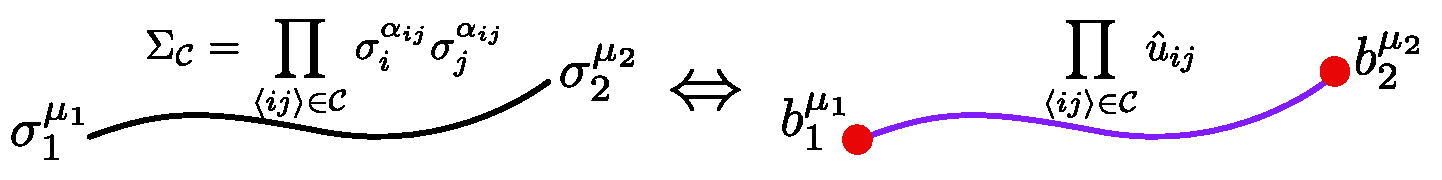
\includegraphics[width=\linewidth]{figures/linking-string-electric-field.pdf}
    \caption{Two $b$-Majorana fermions can also be linked by a series of gauge-field operators, $\prod_{\anglelr{ij}\in\mathcal{C}} \hat{u}_{ij}$. In that way, a physical operator $\xi$ is constructed.}
    \label{fig.linking-strings-electric-field}
\end{figure}
However, the expression \eqref{equ.b-link} only contains $b$-Majorana fermions and cannot be transformed directly to the spin representation. To obtain physical strings containing purely spin operators, we can further insert $c$-Majorana fermions into expression \eqref{equ.b-link}, then we obtain the following result   
\begin{equation}\label{equ.c-b-link}
    b^{\mu_{2n-1}}_{i_{2n-1}}c_{i_{2n-1}} \lr{\prod_{\anglelr{ij}\in\mathcal{C}_{n}} c_i\hat{u}_{ij}c_j}c_{i_{2n}}b^{\mu_{2n}}_{i_{2n}}
\end{equation}
in which those inserted $c$-Majorana fermions are identities $cc=\mathds{1}$, thus everything remains the same. After considering the transformation $\sigma^\mu_i\to ib^\mu_ic_i$, the operator \eqref{equ.c-b-link} is equal to the operators $\xi_n$ defined in the following way
\begin{equation}\label{equ.spin-string-linking-gauge}
    \xi_n \equiv \sigma^{\mu_{2n-1}}_{i_{2n-1}}\Sigma_{\mathcal{C}_n}\sigma^{\mu_{2n}}_{i_{2n}} \quad ; \quad n=1,2,3,\cdots ,L
\end{equation}
up to a phase that depends on the lengths of the strings $\abs{\mathcal{C}_n}$. The process of producing $\xi$-operators from \eqref{equ.b-link} to \eqref{equ.spin-string-linking-gauge} is illustrated in \autoref{fig.linking-strings-electric-field}, analogous to \autoref{fig.linking-strings}. It is straightforward to see that all operators $\xi_n$ defined in a simply-connected subregion $A$ commute with the reduced density matrix $\rho_A$. 
\begin{figure*}
    \centering
    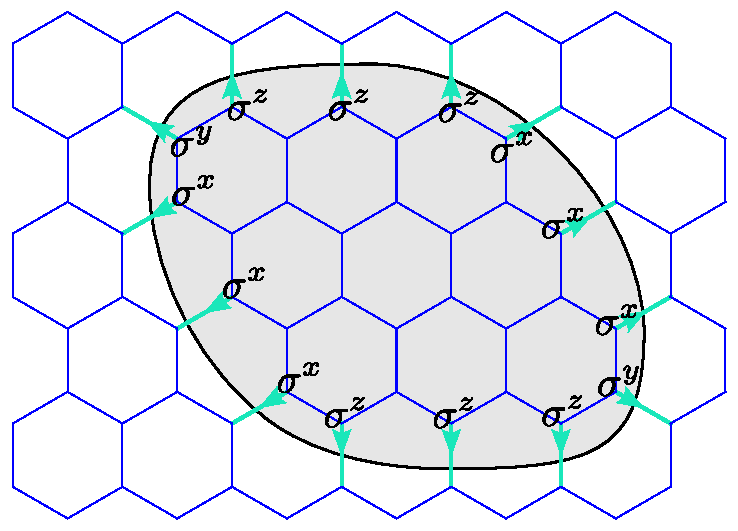
\includegraphics[width=0.24\linewidth]{figures/Yao-Qi-mechanism-origin.pdf}
    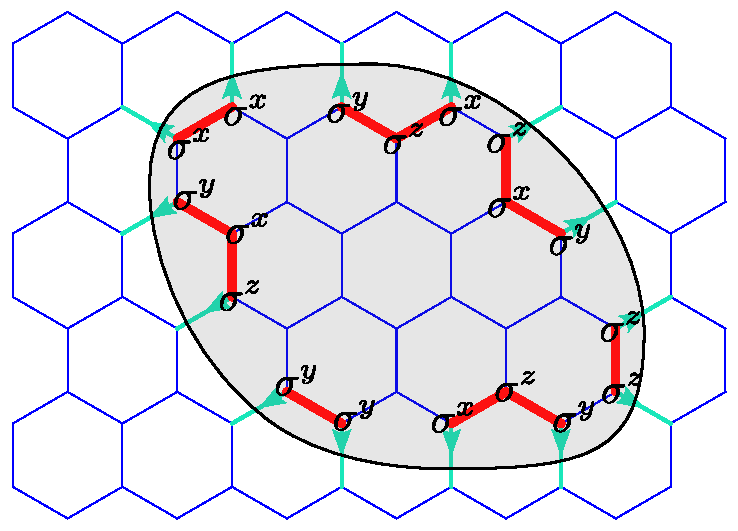
\includegraphics[width=0.24\linewidth]{figures/Yao-Qi-mechanism-dimers.pdf}
    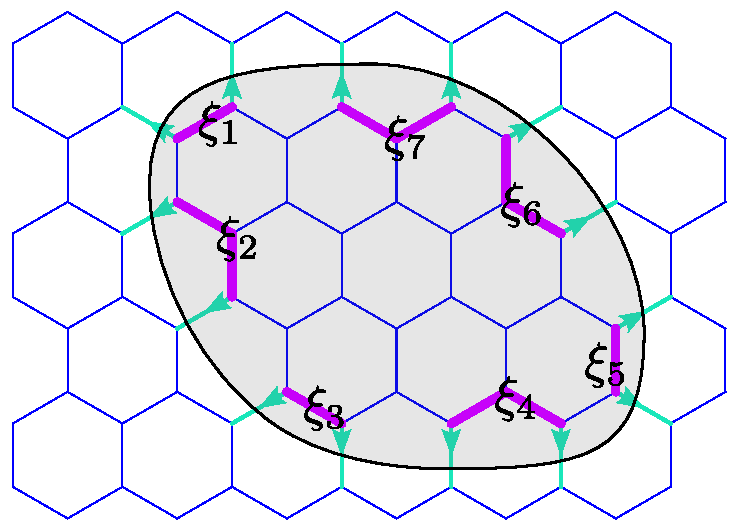
\includegraphics[width=0.24\linewidth]{figures/Yao-Qi-mechanism-xi-def.pdf}
    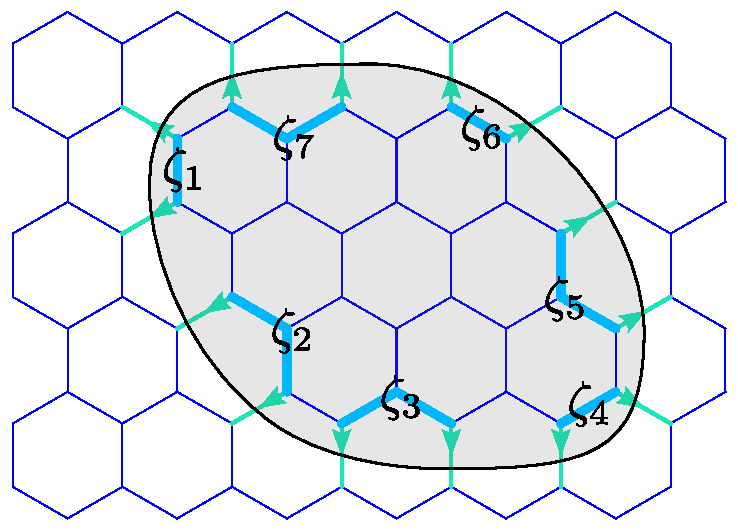
\includegraphics[width=0.24\linewidth]{figures/Yao-Qi-mechanism-zeta-def.pdf}
    \caption{The electric-field operators living on the edges crossing the boundary of the region are split in half, as shown in the first panel. In the physical spin representation, these electric fields correspond to the spin operators $\sigma^\mu$ with directions pointing outwards. The second panel displays string operators that connect two adjacent spins in the first panel in a pair. Multiplying the first panel by the second one gives a series of operators $\xi$, as shown in the third panel. Applying the same method but with the pairing order shifted yields another set of operators $\zeta$, as showcased in the last panel.}
    \label{fig.xi-def}
\end{figure*}
The first three panels of \autoref{fig.xi-def} illustrate an example of the process of defining $\xi$-operators. In the first panel are the spin operators $\sigma^\mu_i$, which are exactly the spin operators shown in equation \eqref{equ.spin-string-linking-gauge}, at the boundary with their directions pointing outwards. In the next panel, we subsequently multiply the string operators $\Sigma_{\mathcal{C}_n}$, which is nothing but the string operator shown in equation \eqref{equ.spin-string-linking-gauge} that lies between the two spin operators residing on the two endpoints of the string, with the spin operators set previously. After that, such operators are used as definitions of $\xi_n$'s, which are illustrated in the third panel of \autoref{fig.xi-def}. In this example, we now focus on $\xi_1$, which is defined as
\[
\xi_1 = \sigma^y_1\lr{\sigma^x_1\sigma^x_2}\sigma^z_2 \propto \sigma_1^z\sigma_2^y.
\]
The subscript ``1'' indicates the lower-left endpoint of the dimer, while ``2'' stands for the other one. It can be shown that $\xi_1$ commutes with every string operator $\Sigma_{\mathfrak{D}}$ with $\mathfrak{D}\subset A$ in a trivial way by examining all possible strings that reach the two endpoints of the dimer where $\xi$ lives. By doing so, one will find that either (i) at one endpoint of a string $\mathcal{C}$, which is right at one of the two endpoints of the $\xi_1$ dimer, is a spin operator whose direction is parallel to the spin operator of $\xi_1$ on that endpoint; Or (ii) none of the two spin operators of $\Sigma_{\mathcal{C}}$, whose positions are the two endpoints of $\xi_1$, is parallel to the spin operator of $\xi_1$ at its position, such that the twice of sign flipping caused by the anti-commutation of Pauli algebra between $\Sigma_{\mathcal{C}}$ and $\xi_1$ gets the positive sign again. These situations, along with the fact that $[\xi_1,W_p]=0\;\forall p$~\footnote{Don't forget that a loop also counts a string, just with two endpoints at the same position. Therefore, proving that every string operator commutes with $\xi_n$ also proves that every plaquette operator commutes with $\xi_n$ at the same time.}, exhaust all the possibilities, allowing us to conclude that $[\xi_1,\rho_A]=0$ because $\rho_A$ consists of plaquette operators and string operators inside $A$, as shown in equation \eqref{equ.red-den-mat-sim-con}. In the same sense, we may generalize this statement to $[\xi_n,\rho_A]=0\;\forall n$, where the operators $\xi_n$ are defined through the process illustrated in \autoref{fig.xi-def} in $A$. At the same time, the regions where $\xi$-operators are supported have no intersection, hence they commute with each other, $[\xi_m,\xi_n]=0\;\forall m,n$. Therefore, the set $\lrg{\xi_1,\cdots,\xi_L}$, with values $\pm 1$, of expectation values of $\xi$-operators defined in $A$ forms good quantum numbers that block-diagonalizes the reduced density matrix $\rho_A$
\begin{equation}\label{equ.rho-block-diagonal-structure}
    \rho_A = \bigoplus_{\lrg{\xi_1,\cdots,\xi_L}} \varrho_{\lrg{\xi_1,\cdots,\xi_L}}
\end{equation}
where each $\varrho_{\lrg{\xi_1,\cdots,\xi_L}}$ is the block labeled by a set of binaries $\lrg{\xi_1,\cdots,\xi_L}$, and thus the number of blocks is $2^{L} = 2^{\abs{\de A}/2}$.

In defining $\xi$-operators, the way we chose to pair points along the boundary was like $(b^{\mu_1}_{i_1},b^{\mu_2}_{i_2}), (b^{\mu_3}_{i_3},b^{\mu_4}_{i_4}),\cdots,(b^{\mu_{2L-1}}_{i_{2L-1}},b^{\mu_{2L}}_{i_{2L}})$. However, it is not the only way to pair these points. We can choose another way in which the pairing order is shifted by one compared to the previous way we adapted for $\xi$-operators
\[
(b^{\mu_2}_{i_2},b^{\mu_3}_{i_3}), (b^{\mu_4}_{i_4},b^{\mu_5}_{i_5}),\cdots,(b^{\mu_{2L}}_{i_{2L}},b^{\mu_1}_{i_1})
\]
and then connect each of them through a new set of strings $\{\mathcal{C}'_n\}$. In this way, a set of operators $\zeta_n$ can be defined
\begin{equation}\label{equ.spin-string-linking-gauge-zeta}
    \zeta_n \equiv \sigma^{\mu_{2n}}_{i_{2n}}\Sigma_{\mathcal{C}'_n}\sigma^{\mu_{2n+1}}_{i_{2n+1}} \quad ; \quad n=1,2,3,\cdots, L
\end{equation}
where the periodic notational convention $i_{2L+1}=i_1$ and $\mu_{2L+1}=\mu_1$ is used. In the same sense, these $\zeta$-operators also commute with the reduced density matrix. An example of a set of $\zeta$-operators is illustrated in the fourth panel of \autoref{fig.xi-def}, from which we can see that the pattern of $\zeta$-operators differs from that of $\xi$-operators by shifting a unit along the boundary, so that each $\xi_n$ is in between $\zeta_{n-1}$ and $\zeta_n$. According to the algebraic rules of Pauli matrices, a relation between $\xi$-operators and $\zeta$-operators can be obtained directly
\begin{equation}\label{equ.xi-zeta-relation}
    \zeta_n\xi_m\zeta_{n} =
\left\{
\begin{array}{ll}
   -\xi_m &;\; \text{for $m=n\vee n+1$} \\
   \xi_m  &;\; \text{otherwise} 
\end{array}
\right.
\end{equation}
This equation implies that the $\zeta$-operators relate different blocks of the density matrix $\rho_A$ in the way that
\begin{equation}\label{equ.related-blocks}
    \zeta_n \varrho_{\lrg{\cdots,\xi_n,\xi_{n+1},\cdots}}\zeta_n = \varrho_{\lrg{\cdots,-\xi_n,-\xi_{n+1},\cdots}}
\end{equation}
By this relation, any two blocks $\varrho_{\lrg{\xi}}$ and $\varrho_{\lrg{\xi'}}$ in $\rho_A$ can be related, and thus their sets of eigenvalues are identical. However, a $\zeta$-operator flips the eigenvalues of two $\xi$-operators at the same time, so it is not quite correct to say any two blocks can be related through applying $\zeta$-operators. Considering this simultaneous flipping of two quantum numbers, the statement should be modified to: Two blocks, $\varrho_{\lrg{\xi}}$ and $\varrho_{\lrg{\xi'}}$, are related by a specific set of $\zeta$-operators only when they have the same total parity, $\prod_{i=1}^{L}\xi_i = \prod_{i=1}^{L}\xi'_i$, defined by multiplying every quantum number in $\lrg{\xi}$.

So far, we have had a better understanding of the block-diagonal structure of $\rho_A$, and now we are going to discuss the origin of the degeneracy in the entanglement spectrum, as well as another point of view of the contribution of the gauge field to the entanglement entropy. Based on the block-diagonal structure \eqref{equ.rho-block-diagonal-structure} of $\rho_A$ and the fact that $\zeta$-operators can relate different blocks to prove them identical, we then conclude that there are 
\[2^{L-1} = 2^{\abs{\de A}/2 - 1}\] 
identical blocks in $\rho_A$. The reason why we only have the number $2^{L-1}$ instead of $2^L$, which is the number of blocks in \eqref{equ.rho-block-diagonal-structure}, is that $\zeta$-operators can only relate blocks with the same parity of the set of quantum numbers $\lrg{\xi}$, so the number of blocks, $2^L$, is actually twice the number of identical blocks. The factor $2^{-1}$ arising from the fixed parity of quantum numbers can also be understood as originating from the exact 1-form Wilson symmetry~\cite{PRX-ent-high}, which is $[\Tilde{W}_h,H] = [\Tilde{W}_v,H] = [W_p,H]=0\;\forall p$. After tracing out the environment $\overline{A}$, the global Wilson operator in the sense of merely the subregion $A$ becomes a string with two endpoints attached to the boundary of $A$, and commutes with $\rho_A$ at the same time. The two endpoints of the Wilson operator can flip the residual $\mathbb{Z}_2$ gauge field at the boundary, playing a role in relating different blocks of $\rho_A$. This is completely the same as the $\zeta$-operators. Based on the block-diagonal structure of $\rho_A$, it can be expressed as
\begin{equation}\label{equ.block-rho-final}
    \rho_A = \bigoplus_{n=1}^{2^{L-1}}\varrho^{(n)}_A
\end{equation}
with all the blocks $\varrho_A^{(n)}$ identical. Substitution of such an expression into the definition of von Neumann entropy directly gives the entanglement entropy, 
\begin{align}\label{equ.EE-from-blocks}
    S_A 
    &= -\Tr_A\rho_A\ln\rho_A \nonumber \\
    &= -\Tr_A\lrm{\bigoplus_{n=1}^{2^{L-1}}\lr{\varrho^{(n)}_A \ln \varrho^{(n)}_A}} \nonumber \\
    &= -2^{L-1}\Tr_A\varrho_A \ln \varrho_A \nonumber \\
    &= -\Tr_A\Tilde{\rho}_A\ln\Tilde{\rho}_A + \lr{\frac{1}{2}\abs{\de A} -  1}\ln 2
\end{align}
where $\Tilde{\rho}_A \equiv 2^{L-1}\varrho_A$ is the normalized density matrix
defined to make $\Tr_A\Tilde{\rho}_A=1$. By comparing Eq.~\eqref{equ.EE-from-blocks} with Eq.~\eqref{equ.EE-separation}, we find that each block $\Tilde{\rho}_A$ corresponds to the Majorana reduced density matrix $\rho_A^F$. At the same time, the gauge part $S^G_A$ can be understood as a measure of the number of identical blocks in $\rho_A$, which is exactly the degree of degeneracy in the entanglement spectrum. This agrees with the gauge nature of such a contribution since the degeneracy arises from the block-diagonal structure of $\rho_A$ along with the fact that every block is identical, and the presence of block-diagonal structure is due to the residual electric field from the Gauss law after the environment is traced out. Notice that the residual Gauss law does not purely cause the degeneracy in the entanglement spectrum. Instead, it also has things to do with the existence of $\zeta$-operators, through which all blocks can be related. Finally, the topological entanglement entropy $-\ln 2$ is a consequence of the constraint that the total parity of the quantum numbers, $\prod_{n=1}^L\xi_n$, is fixed, and its origin lies in the existence of the 1-form Wilson symmetry, which satisfies our earlier understanding about the topological entanglement entropy. The most important thing is that the full entanglement spectrum of the Kitaev ground state is obtained. Since an entanglement spectrum is defined as the spectrum of a reduced density matrix, formula \eqref{equ.block-rho-final} directly answers that the entanglement spectrum is the eigenvalue spectrum of $\varrho_A$ with $2^{\abs{\de A}/2-1}$-fold degeneracy. As shown by the comparison between \eqref{equ.EE-from-blocks} and \eqref{equ.EE-separation}, we know that the block $\varrho_A$ is proportional to the Majorana fermion density matrix $\rho^F_A$, and whose spectrum can be solved exactly using the method proposed in Ref.~\cite{Jin-Korepin, Vidal-Latorre-Rico-Kitaev, Latorre-Rico-Vidal, Peschel_2003, Peschel_2009, Chung_2001, Cheong_2004}.

From a more fundamental point of view, the set of $\xi$-operators block-diagonalizes every string operator in a way identical to what we have for $\rho_A$ because each of them commutes with every string operator, and hence so is $\mathcal{S}^{(A)}_{\mathfrak{D}}$
\[
[\xi_i,\mathcal{S}^{(A)}_{\mathfrak{D}}]=0 \;\forall i\in\lrg{1,2,\cdots,L}
\]
Similar to equation \eqref{equ.block-rho-final}, every $\mathcal{S}$-operator can also be block-diagonalized as
\begin{equation}\label{equ.U-V-block-relation}
    \mathcal{S}^{(A)}_{\mathfrak{D}} = \bigoplus_{n=1}^{2^{L-1}}\mathcal{M}^{(n)}_{\mathfrak{D}}
\end{equation}
where $\{\mathcal{M}^{(n)}_\mathfrak{D}\}$ is a set of identical blocks of $\mathcal{S}^{(A)}_{\mathfrak{D}}$. To ensure that expression \eqref{equ.U-V-block-relation} satisfies rule \eqref{equ.U-rep-algebra}, we also have to implement such an algebraic rule on every block $\mathcal{M}^{(n)}_{\mathfrak{D}}$, 
\[
\mathcal{M}^{(n)}_{\mathfrak{D}}\mathcal{M}^{(n)}_{\mathfrak{D}'} = g(\mathfrak{D},\mathfrak{D}')\mathcal{M}^{(n)}_{\mathfrak{D}\oplus\mathfrak{D}'}
\]
This is reminiscent of \eqref{equ.V-rep-algebra}, which shows that the $\mathcal{M}$-representation is identical to $\mathcal{S}$. Based on this, we then state that those blocks $\mathcal{M}^{(n)}_{\mathfrak{D}}$ in \eqref{equ.U-V-block-relation} are nothing but $\mathcal{M}$-operators defined in \eqref{equ.V-rep-def}. In short, the gauge-field degree of freedom is actually the number of identical blocks of string operators represented by spins, and each identical block depicts the physics of free Majorana fermions. This precisely reflects the fractionalization of the spin degree of freedom into gauge-field and matter sectors, with the matter sector further fractionalizing into deconfined Majorana fermions.


\begin{figure*}
    \centering
    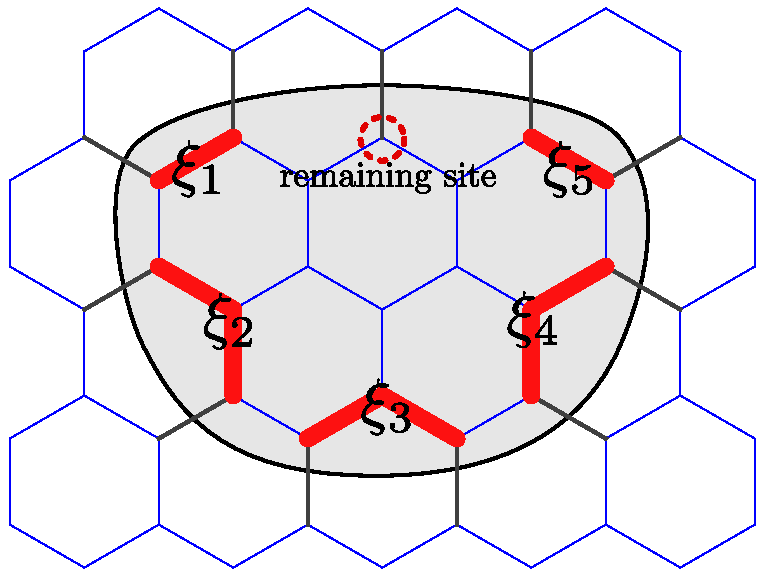
\includegraphics[width=0.25\linewidth]{figures/reshuffle-xi-def-odd.pdf}\hspace{0.5cm}
    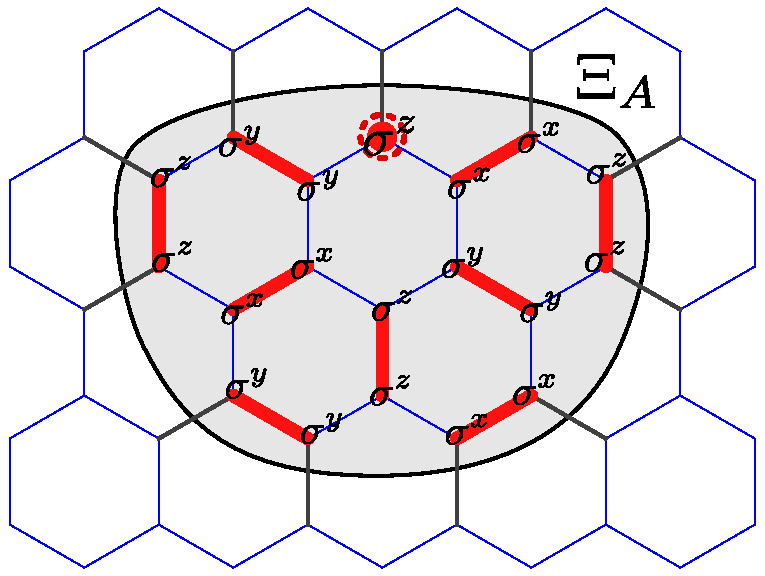
\includegraphics[width=0.25\linewidth]{figures/reshuffle-capital-Xi-def.pdf}\hspace{0.5cm}
    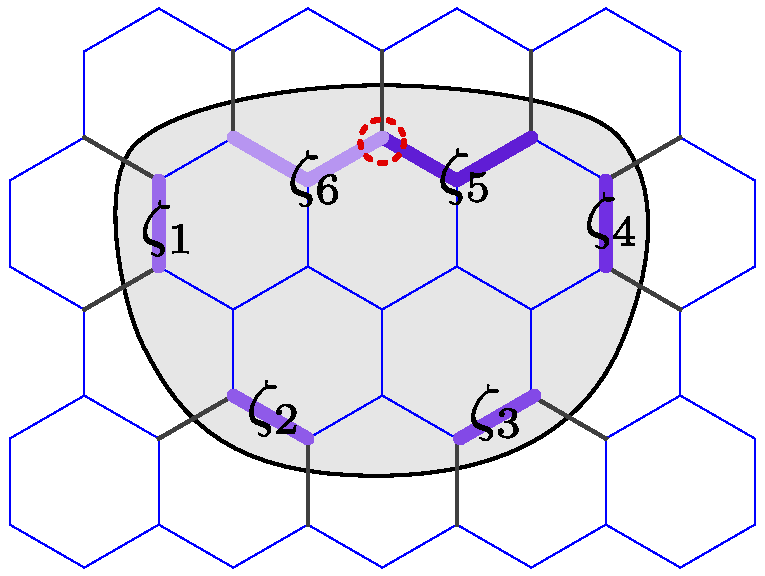
\includegraphics[width=0.25\linewidth]{figures/reshuffle-zeta-def-odd.pdf}
    \caption{For cases with odd $N^A$, there must be a single site $l$ on the boundary that remains unpaired after defining $\xi$-operators by pairing the adjacent edges crossing the boundary, as illustrated in the left-most panel. Based on this phenomenon, we can define an operator $\Xi_A$ in such a way that the remaining site $l$ is filled in with a Pauli matrix $\sigma^\mu_l$, where $\mu$ is the direction of the edge crossing the boundary that connects to $l$. At the same time, the rest of the part is covered by a dimer covering, as illustrated in the middle panel. On the other hand, the $\zeta$-operators are defined in a way similar to what we have introduced, but there are two connected $\zeta$-operators sharing one site, which is exactly $l$ after the pairing we have done to define $\xi$-operators. In the example illustrated in the right-most panel, the two connected $\zeta$-operators are $\zeta_5$ and $\zeta_6$, and we have $\zeta_5\Xi\zeta_5 = \zeta_6\Xi_A\zeta_6 = -\Xi_A$.}
    \label{fig.Xi-odd}
\end{figure*}
In the above discussion, everything is well-defined since $\abs{\de A}$ was set to be even. In that case, the sites along the boundary can be sorted into pairs to define a set of $\xi$-operators that link two sites in a pair. However, as shown by relation \eqref{equ.bulk-boundary-parity}, once the number of lattice sites in $A$ is odd, so is the length of the boundary. This raises an issue that there will always be one single site that remains after sorting lattice sites along the boundary in pairs, as shown in the first panel of \autoref{fig.Xi-odd}. If $L$ is defined as the number of $\xi$-operators, then in cases with odd $\abs{\de A}$, we have
\[
L = \frac{1}{2}\lr{\abs{\de A} - 1}
\]
In this way, the block-diagonal structure \eqref{equ.block-rho-final} and the derivation \eqref{equ.EE-from-blocks} are still valid, but the result should be modified as
\begin{align}\label{equ.EE-odd-blocks}
    S_A &= -\Tr_A\Tilde{\rho}_A\ln\Tilde{\rho}_A + \lr{L-1}\ln 2 \nonumber\\
    &= -\Tr_A\Tilde{\rho}_A\ln\Tilde{\rho}_A + \lr{\frac{1}{2}\abs{\de A}-\frac{3}{2}}\ln 2
\end{align}
where $\Tilde{\rho}_A\equiv 2^{L-1}\varrho_A$. The form of \eqref{equ.EE-odd-blocks} is the same as that of \eqref{equ.EE-odd-derive-1}, showing that the block $\Tilde{\rho}_A$ here is identical to the Majorana reduced density matrix \eqref{equ.rho-A-F-odd} with a redundant Majorana fermion included. 

In Section~\ref{sec:EE-calculation-odd}, the result of the Majorana entanglement spectrum shows that the degree of degeneracy is 
\[
2^{\frac{N^A+1}{2}-N^A_p} = 2^{\frac{1}{2}\lr{\abs{\de A} - 1}} = 2^L
\]
However, according to the discussion in the previous part for cases with an even number of sites, the degree of degeneracy is $2^{L-1}$ if there are $L$ well-defined $\xi$-operators. This discrepancy between counting the number of $\xi$-operators and analyzing the degree of degeneracy according to the Majorana entanglement spectrum implies that, apart from the set of $\xi$-operators, there exists an additional operator that further block-diagonalizes $\rho_A$ to give an additional 2-fold degeneracy to the entanglement spectrum. At the end of Section~\ref{sec:EE-calculation-odd}, we have elucidated that the additional 2-fold degeneracy in the entanglement spectrum of the Majorana sector originates from the total fermion parity, in the sense that $\rho_A$ is further block-diagonalized into two identical blocks by $\hat{\bog{\pi}}^{(A)}$, corresponding to even and odd, respectively. Therefore, we anticipate that the additional operator, which will be denoted by $\Xi_A$ later on, is related to the total fermion parity in the Majorana representation. A feasible choice is a dimer covering of the subregion $A$. In that matter, $\Xi_A$ is defined as
\begin{equation}\label{equ.Xi-def}
    \Xi_A \equiv \sigma^\mu_l \prod_{\anglelr{ij}\in\mathfrak{D}_{\mrm{DC}}^{A(l)}}\dimer{i}{j}
\end{equation}
The edge configuration $\mathfrak{D}_{\mrm{DC}}^{A(l)}$ stands for a dimer covering of $A$ with a site $l$ being excluded. Since $N^A$ is an odd number, it is not possible for a dimer configuration composed of non-overlapping dimers to cover the entire subregion. The dimer covering is not uniquely defined. A dimer configuration can be arbitrarily chosen as long as $\Xi_A$ gives the 2-fold degeneracy in the entanglement spectrum. The remaining site $l$ is required to be at the boundary of the subregion $A$, which will be explained later, and at which the direction $\mu$ of the Pauli matrix $\sigma_l^\mu$ is that of the edge connected to $l$ that crosses the boundary. An example is illustrated in \autoref{fig.Xi-odd}, where the remaining site $l$ is in the upper portion of the subregion. 

$\Xi_A$ can be examined to commute with $\rho_A$ in the same way as used for $\xi$-operators. String operators are composed of multiple dimers, and every dimer commutes with the dimer covering because of the properties of Pauli matrices. Therefore, the only thing to be concerned about is $\sigma^\mu_l$ lying at the remaining site.
As we have defined, the site $l$ is at the boundary and $\mu$ points outward, it can be seen directly that, inside $A$, there are only two edges connected to $l$, and the corresponding string operator of both edges anti-commutes with $\sigma^\mu_l$. However, since the string operator also anti-commutes with the dimer that connects to the other endpoint of the edge, the two anti-commutations cancel each other. In the end, every string operator with $\mathfrak{D}\subset A$ commutes with $\Xi_A$. Finally, because $\rho_A$ is composed of string operators inside $A$, we conclude that $[\Xi_A,\rho_A]=0$. 

It would be transparent to see that $\Xi_A$ is related to the total fermion parity by transforming \eqref{equ.Xi-def} into the Majorana fermion representation, and we find that it is equal to the total fermion parity operator multiplied by the gauge-field operators arranged in order of the dimer covering $\mathfrak{D}^{A(l)}_{\mrm{DC}}$
\[
\Xi_A \propto \lr{\prod_{\anglelr{ij}\in  \mathfrak{D}^{A(l)}_{\mrm{DC}}} \hat{u}_{ij}} \lr{b^\mu_l\prod_{i\in A}c_i}
\]
up to a phase. In the above formula, the total fermion parity operator is defined as
\begin{equation}\label{equ.total-fermion-parity-odd}
    \hat{\bog{\pi}}^{(A)} \propto b^\mu_l\prod_{i\in A}c_i
\end{equation}
with a phase correction depending on the geometry of the subregion. Because the gauge has been fixed as $u_{ij}=1\;\forall\anglelr{ij}$, the expectation value of $\Xi_A$ is completely determined by that of $\hat{\bog{\pi}}^{(A)}$. The definition of the total fermion parity here is different from what we encountered in \eqref{equ.total-fermion-parity-entire-system} and \eqref{equ.total-fermion-parity-Sigma-Z}. In fact, it is due to $N^A$ being an odd number, so that $\prod_{i\in A}c_i$ itself only contains an odd number of Majorana fermions, hence not sufficient to define a fermion parity operator. This mechanism has been discussed in Section~\ref{sec:EE-calculation-odd}, and the alternative we adopted there is to include a redundant Majorana fermion $c_{(N^A+1)}$. In \eqref{equ.total-fermion-parity-odd}, it can be seen that the redundant fermion is in fact $b^\mu_l$ borrowed from the gauge sector. The situation in which the $c$-Majorana sector borrows a Majorana fermion from the gauge sector is also demonstrated in the derivation procedures \eqref{equ.EE-odd-derive-1} and \eqref{equ.EE-reduce}. By now, the physical meaning of the redundant fermion and its origin are clearly reflected by $\Xi_A$. 

So far, we have $L$ distinct $\xi$-operators and $\Xi_A$ that commute with $\rho_A$. These operators give $2^{L+1}$ blocks labeled with a set of eigenvalues $\lrg{\xi_1,\cdots,\xi_L;\Xi_A}$. To prove that these blocks are identical, leading to extensive degeneracy, we also have to find $(L+1)$ $\zeta$-operators that relate all the blocks in the same way as \eqref{equ.xi-zeta-relation}. In the line of defining $\xi$-operators, we can only define $L$ $\zeta$-operators. However, it turns out that we can still find $(L+1)$ $\zeta$-operators since they are not required to commute with each other. As illustrated in the last panel of \autoref{fig.Xi-odd} the arrangement of $\zeta$-operators is designed in such a way that two of them overlap at the remaining site $l$. In this way, the $\xi$-operators can still be flipped through \eqref{equ.xi-zeta-relation}. More importantly, both overlapping $\zeta$-operators can flip the sign of $\Xi_A$. In \autoref{fig.Xi-odd}, these two operators are $\zeta_5$ and $\zeta_6$, by which $\Xi_A$ can be flipped in the way that $\zeta_5\Xi_A\zeta_5 = \zeta_6\Xi_A\zeta_6 = -\Xi_A$. In all, the situation here is similar to what we encountered in cases with even $N^A$, in which each $\zeta$-operator simultaneously flips two values in the set $\lrg{\xi_1,\cdots,\xi_L;\Xi_A}$. Therefore, although we have $2^{L+1}$ operators to block-diagonalize $\rho_A$, they only provide $2^L$-fold degeneracy in the entanglement spectrum. This agrees with our analysis in Section~\ref{sec:EE-calculation-odd}, and the operator $\Xi_A$ indeed gives a 2-fold degeneracy to the entanglement spectrum. 

It seems that $\Xi_A$ can also be defined in cases with even $N^A$ as illustrated in \autoref{fig.dimer-covering}, and gives a 2-fold degeneracy as well.
\begin{figure}
    \centering
    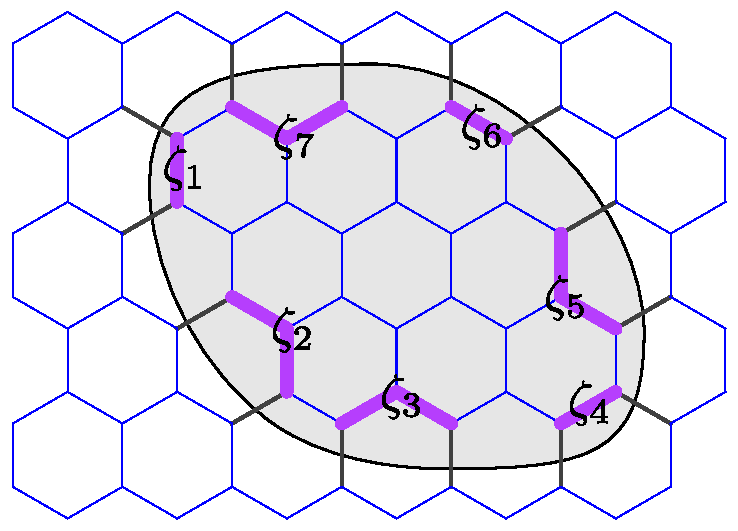
\includegraphics[width=0.4\linewidth]{figures/reshuffle-larger-zeta.pdf}\hspace{0.5cm}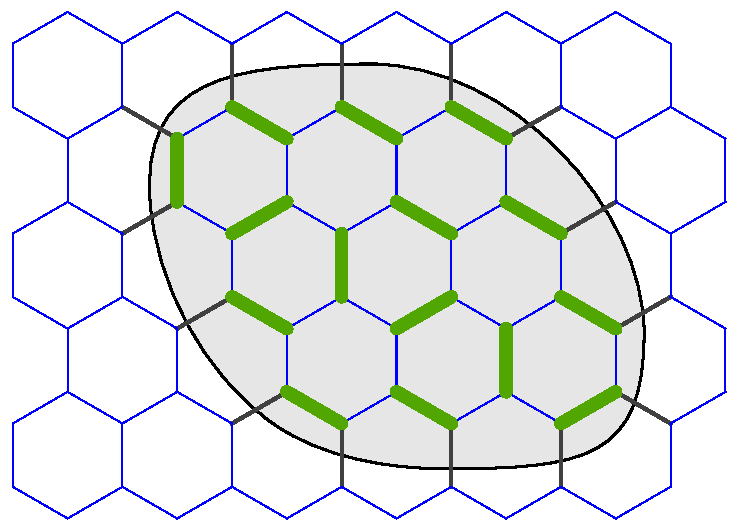
\includegraphics[width=0.4\linewidth]{figures/reshuffle-larger-dimer-covering.pdf}
    \caption{For regions with an even number of lattice sites, at least a dimer covering is well defined, like the one illustrated in the right panel. Assigning a string operator to each dimer in the configuration gives a dimer-covering string operator $\Xi_A$ without a single unpaired site, unlike we encountered in cases with an odd number of sites. However, it can be directly checked that $\Xi_A$ in this case commutes with every $\zeta$-operator. Therefore, such an operator doesn't provide additional degeneracy in the entanglement spectrum.}
    \label{fig.dimer-covering}
\end{figure}
In this case, the pattern is simply a dimer covering without a remaining site. However, $\Xi_A$ defined in this case commutes with every $\zeta$-operator, implying that no operator can relate blocks with $\Xi_A=+1$ to $\Xi_A=-1$ and vice versa. Thus, $\Xi_A$ cannot provide a 2-fold degeneracy in the entanglement spectrum in cases with even $N^A$. This constitutes an intrinsic difference between cases with even and odd $N^A$, which is reflected in the total fermion parity in the subregion in the Majorana representation, or equivalently in the dimer covering operator $\Xi_A$ in the physical spin formulation.

\section{Summary and Discussions}

In this work, we derive the explicit form of the density matrix of the Kitaev ground state on a torus and discuss the entanglement information encoded therein in detail. We use the spin formulation throughout this paper to address the lack of a spin-language–based theoretical understanding of quantum spin systems, whose fundamental constituents are the spins themselves 

This work can be summarized in three main results. First, the ground state density matrix is composed of string operators in different edge configuration equivalent classes. The structure of the equivalence class arises from the flux-free property of the ground state, in the sense that edge configurations that can be related by loops are sorted into an equivalence class. Regardless of the fermion parity condition, an equivalence class is only hinged on the pattern of endpoints of the edge configurations therein. This structure shows the equivalence between the spin representation and the fermion representation of edge configurations. 

Second, a reduced density matrix of a simply-connected subregion is obtained. The calculation of the entanglement entropy implies that it is composed of identical blocks, and each block is the density matrix of the corresponding free-fermion system. In other words, the entanglement spectrum has an extensive degeneracy, and the distinct values in the entanglement spectrum are the ones in the entanglement spectrum of the equivalent free-fermion system. The gauge-field contribution to the entanglement entropy is actually the measure of the degeneracy in the entanglement spectrum. We also investigated the issue raised by cases with an odd number of lattice sites. Our approach solves this subtlety by borrowing a Majorana fermion from the gauge sector, and this derivation also leads to the finding of an additional 2-fold degeneracy in the entanglement entropy of the fermion sector.

Third, inspired by~\cite{PRX-ent-high}, the block-diagonal structure of the reduced density matrix is directly proven. The physical picture is based on the \textit{residual} Gauss law of the gauge theory after the environment is traced out, and it then serves as real symmetries that give good quantum numbers for block-diagonalizing the reduced density matrix. After that, the blocks are proven to be identical because the exact 1-form Wilson symmetry relates all the blocks together. Since the gauge theory of the Kitaev model is only an emergent structure in the enlarged parton space, the fractionalized fermions need to be \textit{glued} back into physical spin degrees of freedom by inserting strings that connect pairs of Majorana fermions. Lastly, a global operator defined in the sense of dimer coverings that reflects fermion parity in the subregion is found to give an additional 2-fold degeneracy when the number of lattice sites is odd, in agreement with the 2-fold degeneracy found in the Majorana fermion sector.

We would like to mention that the form of the density matrix~\eqref{equ.density-matrix} is reminiscent of the tensor network state proposed by~\cite{string-gas-TN}, in which the tensor network \textit{Ans\"atze} that approximates the Kitaev ground state is constructed by applying a tensor product operator to an initial state. The tensor product operator is composed of a \textit{loop gas} operator and a \textit{dimer gas} operator, in which the loop gas term is exactly the plaquette projector~\eqref{equ.p-projector}, and the dimer gas part consists of low-order terms of the summation in \eqref{equ.density-matrix}. The similarity between these two might be due to the projector nature of a pure state density matrix. If the tensor-product operator approximately captures the density matrix of the ground state, this might explain the remarkably good agreement between the results of \cite{string-gas-TN} and the exact solution.

Another remark is that the theoretical framework proposed in this work is general for every \textit{Kitaev-like} model, as long as it is exactly solvable in a way similar to the Kitaev model, in which $\mathbb{Z}_2$ fluxes have no dynamics, and the spin Hamiltonian can be completely separated into $\mathbb{Z}_2$ gauge fields and the Majorana matter parts. For example, the Kitaev model has been generalized in the way that three-spin interaction terms are included~\cite{3-spin-1, 3-spin-2, 3-spin-3, 3-spin-4, Xiang-3-spin-chiral}. The three-spin term gives rise to a time-reversal-symmetry-breaking next-nearest-neighbor Majorana hopping in the Majorana representation similar to the Haldane model~\cite{Haldane-model}, giving a chiral ground state with a non-zero Chern number. The form of the density matrix proposed in this work should also be valid for Kitaev-like models with different lattice geometries, such as the Yao-Kivelson model, which can host a chiral-spin-liquid ground state~\cite{yao-kivelson}. The lattice structure in the Yao-Kivelson model is composed of triangular and dodecagonal plaquettes, for which the corresponding plaquette operators can be defined similarly in the Kitaev model, and the pattern of the equivalence class, as well as the correspondence between strings and Majorana fermions, might still be there. If this conjecture is correct, then we could write down an explicit form of the density matrix of a chiral spin liquid formulated in terms of spin operators, which might provide a new point of view based on a spin formulation to understand the topological structure in a chiral spin liquid traditionally characterized by the Chern number in the single-particle picture.

\section*{Acknowledgments}
\alert{ask}

\appendix

\section{Explicit Calculation of Reduced Density Matrices}\label{appendix:reduced-density0matrix}
We follow the general reduced density matrix of a simply-connected region $A$ and continue to carry out the partial trace explicitly to derive the reduced density matrix. Instead of isolating $\prod_{p\in A}\lr{\mathds{1}+W_p}$ at the beginning, it is clearer to see what terms survive after tracing out the environment if we include the whole part of the density matrix while calculating the trace. Both $\mathcal{P}^{(p)}$ and $\mathcal{P}^{(p)}_A$ are projectors, and $\mathcal{P}^{(p)}$ is a projector onto a subspace of the Hilbert space to which $\mathcal{P}^{(p)}_A$ projects. From this observation, we can duplicate the projector $\mathcal{P}^{(p)}_A$ as a redundant term: $\mathcal{P}^{(p)} = \mathcal{P}^{(p)}\mathcal{P}^{(p)}_A$. Therefore, the reduced density matrix of a simply-connected region $A$ can be written as
\begin{align*}
\rho_A &= \frac{1}{2^{N-N_p+2}}\Tr_{\overline{A}}\lrm{\mathcal{P}^{(p)}_A\mathcal{P}^{(p)}\sum_{[\mathfrak{D}]}\mathfrak{C}_\mathfrak{D}\Sigma_\mathfrak{D}} \\
&= 
\frac{1}{2^{N+2}}\mathcal{P}_A^{(p)} \sum_{[\mathfrak{D}]}\mathfrak{C}_\mathfrak{D} \Tr_{\overline{A}}\lrm{\prod_{p}\lr{\mathds{1}+W_p}\Sigma_\mathfrak{D}}
\end{align*}
After that, we investigate what terms can survive after the following trace,
\begin{align*}
    &\sum_{[\mathfrak{D}]}\mathfrak{C}_{\mathfrak{D}}\Tr_{\overline{A}}\lrm{\prod_{p}\lr{\mathds{1} + W_p}\Sigma_{\mathfrak{D}}}\\
=&
2\sum'_{\mathcal{A}}\sum_{[\mathfrak{D}]}\mathfrak{C}_{\mathfrak{D}} \Tr_{\overline{A}}\lrm{ \lr{\prod_{p\in\mathcal{A}}W_p }\Sigma_{\mathfrak{D}}}
\end{align*}
As a reminder, we denote by $\mathcal{A}$ the sets of plaqettes as defined in \eqref{equ.lattice-Stokes}. Since only two types of terms survive after taking the trace, which are those with (i) $\mathcal{A}\subset A$ and $[\mathfrak{D}]\subset A$ and (ii) $\mathcal{A}\oplus\mathfrak{P}\subset A$ and $[\mathfrak{D}\oplus\mathfrak{D}_Z]\subset A$, respectively. Both give the same contribution. The reduced density matrix is therefore
\begin{align*}
&2\sum'_{\mathcal{A}}\sum_{[\mathfrak{D}]}\mathfrak{C}_{\mathfrak{D}} \Tr_{\overline{A}}\lrm{ \lr{\prod_{p\in\mathcal{A}}W_p } \Sigma_{\mathfrak{D}}} \\
=& 2\prod_{p\in A}\lr{\mathds{1}+W_p}\lrm{ 2\sum_{[\mathfrak{D}]\subset A} \mathfrak{C}_{\mathfrak{D}}\Sigma_{\mathfrak{D}} 
}
\Tr_{\overline{A}}\lr{\mathds{1}_{\overline{A}}} \\
=& \mathcal{P}^{(p)}_A 2^{N-N^A+N^A_p+2} \sum_{[\mathfrak{D}]\subset A} \mathfrak{C}_{\mathfrak{D}}\Sigma_{\mathfrak{D}}
\end{align*}
Substituting this result back into the density matrix, we finally have
\begin{equation}\label{GeneralReducedDensityMatrix_first.e}
  \rho_A = \frac{1}{2^{N^A-N^A_p}}\mathcal{P}^{(p)}_A \sum_{[\mathfrak{D}]\subset A}\mathfrak{C}_\mathfrak{D} \Sigma_{\mathfrak{D}}
\end{equation}
The result is in agreement with \eqref{equ.red-den-mat-sim-con}, which has been verified to be properly normalized and to yield correct expectation values for observables.

\section{Fermion Representation of the Density Matrix}\label{appendix:Majorana-derivation}
The ground state of Hamiltonian \eqref{equ.MF-Hamiltonian} reads~\cite{Yao-Qi}
\begin{equation}\label{equ.fermion-state}
    \ket{\psi} = \sqrt{2^{N-1}} \mathcal{P}_G\ket{u}\ket{M}
\end{equation}
The Gutzwiller projector $\mathcal{P}_G=\prod_{i}\lr{\frac{\mathds{1}+D_i}{2}}$ implements the Gauss law of the $\mathbb{Z}_2$ gauge theory in the Majorana representation of the Kitaev model, and $D_i = b^x_ib^y_ib^z_i c_i$ is the generator of the $\mathbb{Z}_2$ gauge transform. The Gutzwiller projector can also be expanded in the following way~\cite{projector-1, projector-2, Fu-Knolle-Perkins-2018}
\[
\mathcal{P}_G = \prod_{i}\lr{\frac{\mathds{1} + D_i}{2}}= \frac{1}{2^{N-1}}\lr{\frac{\mathds{1} + \prod_iD_i}{2}}\sum_{\lrg{i}}'\prod_{j\in\lrg{i}}D_j
\]
where the primed sum stands for a summation over subsets $\lrg{i}$ with sizes smaller than half of the system, $\abs{\lrg{i}}\leq N/2$. The coefficient $\sqrt{2^{N-1}}$ in the state \eqref{equ.fermion-state} is the factor that normalizes the state
\begin{align*}
    \sbraket{\psi}{\psi} &= 2^{N-1}\bra{M}\bra{u}\mathcal{P}_G\ket{u}\ket{M} \\
    &= \bra{M}\bra{u}\lr{\frac{\mathds{1} + \prod_iD_i}{2}}\sum_{\lrg{i}}'\prod_{j\in\lrg{i}}D_j\ket{u}\ket{M} \\
    &= \sum_{\lrg{i}}'\bra{M}\bra{u}\prod_{j\in\lrg{i}}D_j\ket{u}\ket{M} \\
    &= 1
\end{align*}
In the last second line, we used a fact that the state $\ket{u}\ket{M}$ is intrinsically an eigenvector of the operator $\prod_i D_i$ with eigenvalue $+1$. This operator is $\mathbb{Z}_2$ and commutes with the Hamiltonian; therefore, the state $\ket{u}\ket{M}$ is an eigenvector with eigenvalue $\pm 1$. The projector $\lr{\frac{\mathds{1}+\prod_iD_i}{2}}$, hidden in the Gutzwiller projector, selects only the states with eigenvalue $ +1$. Therefore, we only pick the state $\ket{u}\ket{M}$ with the eigenvalue $+1$. As for the last line of the derivation, we know that $D_i$ is the generator of the $\mathbb{Z}_2$ gauge transform and can flip the gauge fields residing on the three edges connected to the site $i$, which implies that the state $D_i\ket{u}$ is orthogonal to the original state $\ket{u}$ before being flipped, so only the term $\lrg{i}=\varnothing$ survives in the summation. It is worth mentioning that the operator is nothing but the fermion parity operator $\hat{\bog{\pi}}$ multiplied with all of the gauge field operators up to a phase~\cite{projector-1}
\[
\prod_i D_i = \prod_ib^x_ib^y_ib^z_ic_i \propto \prod_{\anglelr{ij}}b^{\alpha_{ij}}_{i}b^{\alpha_{ij}}_j\prod_ic_i \propto \lr{\prod_{\anglelr{ij}}\hat{u}_{ij}}\hat{\bog{\pi}}
\]
The phase could be $\pm 1$, depending on the boundary condition of the system~\cite{projector-1, projector-2}. Since $\ket{u}$ is the eigenvector of gauge field operators $\hat{u}_{ij}$ and $\ket{M}$ is the eigenvector of $\hat{\bog{\pi}}$ as the total fermion parity is fixed, it is natural that the state $\ket{u}\ket{M}$ is the eigenvector of the operator $\prod_i D_i$ with the eigenvalue $\pm 1$.

The density matrix of the ground state is a pure state of $\ket{\psi}$
\[
\rho = \ket{\psi}\bra{\psi} = 2^{N-1}\mathcal{P}_G \lr{\ket{u}\bra{u}\otimes\ket{M}\bra{M}} \mathcal{P}_G
\]
The gauge part $\ket{u}\bra{u}$ is nothing but a projector onto the state $\ket{u}$ obtained by fixing the gauge. As usual, for a ground state, the gauge can be fixed trivially as $u_{ij}=+1\forall\anglelr{ij}$. Thus, the projector $\ket{u}\bra{u}$ in such a gauge can be expressed as
\begin{equation}
    \ket{u}\bra{u} = \prod_{\anglelr{ij}}\lr{\frac{\mathds{1} + \hat{u}_{ij}}{2}}
\end{equation}
The projector $\ket{M}\bra{M}$ is the density matrix of the ground state of the effective free Majorana fermion system, and is denoted by $\ket{M}\bra{M}=\rho^F$ in the main part of this paper. The density matrix $\rho^F$ only contains the information of $c$-Majorana fermions, and can be expressed in terms of those $c$-Majorana fermion operators, whose form has been shown in equation \eqref{equ.rho-F}. Combining these results, we ultimately obtain the density matrix of the ground state
\begin{equation}\label{equ.Majorana-density-matrix}
    \rho = 2^{N-1}\mathcal{P}_G\prod_{\anglelr{ij}}\lr{\frac{\mathds{1} + \hat{u}_{ij}}{2}} \rho^F \mathcal{P}_G
\end{equation}
Our goal in this section is to derive the spin representation of the density matrix, so we must find a way to transform the Majorana fermion operators back into spin operators. Here, we apply the following transformation
\[
\dimer{i}{j} = \mathcal{P}_G \hat{u}_{ij}ic_jc_i \mathcal{P}_G = \mathcal{P}_G\hat{u}_{ij}ic_jc_i,
\]
where we have applied the fact that $ib^\mu_ic_i$ commutes with the $\mathbb{Z}_2$ gauge generator, thus $[ib^\mu_i c_i, \mathcal{P}_G]=0$. In general, the above relation implies the direct correspondence between $\Sigma_\mathfrak{D}$ and $\mathcal{M}_\mathfrak{D}$
\begin{equation}\label{equ.U-V-relation} 
\mathcal{P}_G
    \lr{\prod_{\anglelr{ij}\in\mathfrak{D}}\hat{u}_{ij}} \mathcal{M}_\mathfrak{D} = \Sigma_{\mathfrak{D}}\mathcal{P}_G
\end{equation}
The Gutzwiller projection of the last term is actually redundant since $\Sigma_{\mathfrak{D}}$ is already physical. We add this here to emphasize that we restrict ourselves to physical space. With this equation, the gauge part, composed of gauge-field operators, can then be represented in terms of $\Sigma_\mathfrak{D}$ and $\mathcal{M}_\mathfrak{D}$. Therefore, equation \eqref{equ.Majorana-density-matrix} can be rewritten as
\begin{align*}
    \rho &= \frac{2^{N-1}}{2^{3N/2}} \sum_{\mathfrak{D}} \mathcal{P}_G \lr{\prod_{\anglelr{ij}\in\mathfrak{D}} \hat{u}_{ij}} \rho^F \mathcal{P}_G \\
    &=\frac{1}{2^{N/2+1}} \sum_{\mathfrak{D}} \Sigma_\mathfrak{D} \mathcal{P}_G \mathcal{M}_\mathfrak{D} \rho^F\mathcal{P}_G
\end{align*}
Where the denominator $2^{3N/2}$ in the first line arises from the gauge field projector and the fact that the number of edges of a honeycomb lattice is three half that of the lattice sites. The Majorana part in the last line can be further simplified by expressing the Majorana density matrix using equation \eqref{equ.rho-F} and 
\[
\mathcal{P}_G \mathcal{M}_\mathfrak{D} \mathcal{P}_G =
\left\{
    \begin{array}{ll}
        \mathcal{P}_G & ;\;\text{if $\mathfrak{D}\sim \varnothing$} \\
        0 & ;\;\text{otherwise}
    \end{array}
\right.
\] 
because $\mathcal{M}_\mathfrak{D}$ is physical only when $\mathfrak{D}\sim\varnothing$. So,
\begin{align*}
    \mathcal{P}_G \mathcal{M}_\mathfrak{D} \rho^F\mathcal{P}_G &= \frac{1}{2^{N/2}} \sum_{[\mathfrak{D}']} \mathfrak{C}_{\mathfrak{D}'} \mathcal{P}_G \mathcal{M}_\mathfrak{D} \mathcal{M}_{\mathfrak{D}'} \mathcal{P}_G \\
    &= \frac{1}{2^{N/2}}\sum_{[\mathfrak{D}']} g(\mathfrak{D},\mathfrak{D}') \mathfrak{C}_{\mathfrak{D}'} \mathcal{P}_G \mathcal{M}_{\mathfrak{D}\oplus\mathfrak{D}'} \mathcal{P}_G \\
    &= \frac{1}{2^{N/2}} \mathfrak{C}_{\mathfrak{D}} \mathcal{P}_G
\end{align*}
Notice that the factor $g(\mathfrak{D},\mathfrak{D})=+1$ when the number of $A$-sublattice points and that of $B$-sublattice points in $\mrm{EP}(\mathfrak{D})$ are identical. Otherwise, it will be equal to $-1$. We simply reduce $g(\mathfrak{D},\mathfrak{D})$ to $+1$ directly because only those configurations satisfying $g(\mathfrak{D},\mathfrak{D})=+1$ have finite values of $\mathfrak{C}_\mathfrak{D}$. Combining this result with the density matrix obtained previously, we get
\begin{equation}\label{equ.spin-rho-from-fermion}
    \rho = \frac{1}{2^{N+1}} \sum_{\mathfrak{D}} \mathfrak{C}_\mathfrak{D} \Sigma_\mathfrak{D} 
\end{equation}
The Gutzwiller projector has been omitted because we now completely restrict ourselves to physical space. The normalization factor is $2^{-N-1}$ instead of $2^{-N}$ because two different edge configurations $\mathfrak{D}_Z\oplus\mathfrak{D}$ and $\mathfrak{D}_{zz}\oplus\mathfrak{D}$ give the identical string operator $\Sigma_{\mathfrak{D}_Z\oplus\mathfrak{D}} = \Sigma_{\mathfrak{D}_{zz}\oplus\mathfrak{D}}$ for any $\mathfrak{D}$, as explained in Section~\ref{sec:density-matrix-whole}. Thus, the summation should be divided by two to avoid double-counting. Notice that we do not have this issue in $\rho^F$ since $\mathcal{M}_{\mathfrak{D}_Z}$ is not identical to $\mathcal{M}_{\mathfrak{D}_{zz}}$, which is proportional to identity $\mathcal{M}_{\mathfrak{D}_{zz}}\propto\mathds{1}$. Therefore, we have to treat them as two different components, and both should be included in $\rho^F$. After grouping the terms in \eqref{equ.spin-rho-from-fermion} into equivalence classes, it will eventually reproduce \eqref{equ.density-matrix}. 

\section{Proof of Eq.~\eqref{equ.Pick_sim-con}}\label{appendix:Pick}
\begin{figure}
    \centering
    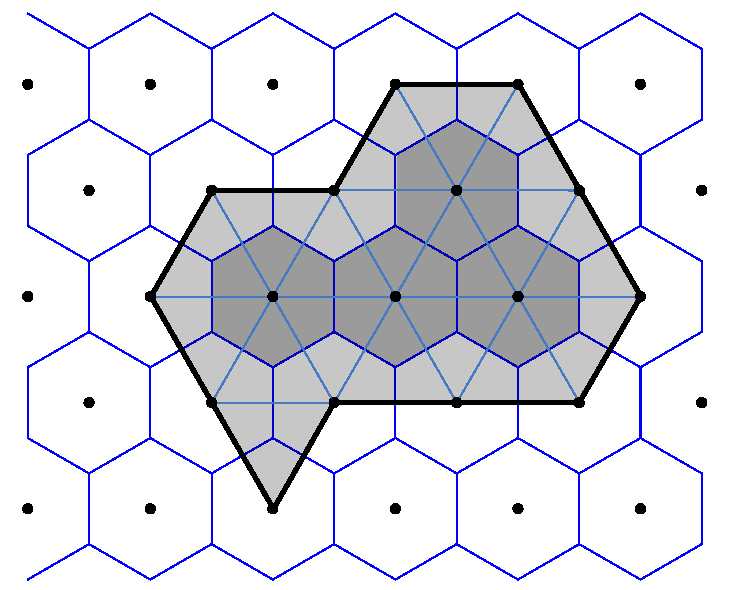
\includegraphics[width=0.6\linewidth]{figures/dual-lattice-Pick-theorem.pdf}
    \caption{A triangle lattice and a honeycomb lattice are dual to each other, in the sense that each lattice point of a system is at the center of a face of the other one. The boundary $C=\de A$ of the shaded region $A$ is a \textit{circuit} defined in the triangle lattice. As shown above, $A$ is composed of $f$ faces of the triangular lattice, in which each face corresponds to a vertex of the dual honeycomb lattice, indicating $f=N^A$. The darker shaded region is composed of $N^A_p$ hexagons entirely inside $A$, which is identical to counting the number of vertices $v$ of the triangular lattice circled by $C$. The length $\ell\equiv\abs{C}$ of the circuit can be understood as the number of edges in the honeycomb lattice that cross $C$. }
    \label{fig.dual-lattice-Pick-theorem}
\end{figure}
We find it more convenient to prove the formula by mapping the original honeycomb lattice to its dual triangular lattice, because a theorem on this problem has been discussed for triangular lattices~\cite{flux-2}. 

A \textit{circuit} $C$ of length $\ell$ in a lattice is defined as an ordered sequence of distinct sites $i_1,\cdots, i_\ell$ with the periodic property that $(i_n, i_{n+1})$ is an edge for $n = 1, \cdots, \ell$ with $i_{\ell+1} \equiv i_1$, and the area enclosed by $C$ is denoted by $A$, which is simply-connected. Consider a triangular lattice. Lemma 2.3 of~\cite{flux-2} gives the following equation
\begin{equation}\label{equ.Lieb-Loss-formula}
    \ell = f - 2v + 2
\end{equation}
where $f$ and $v$ denote the number of interior \textit{faces} and \textit{vertices} of $A$, respectively, and $\ell\equiv\abs{C}$ is the length of the circuit. See \autoref{fig.dual-lattice-Pick-theorem} for an illustration. In the figure, it is also clearly shown that the dual lattice of a triangular lattice is a honeycomb lattice, which is the geometry of our interest in this work. The duality gives several correspondences between the triangular and honeycomb lattices, which are $\ell\leftrightarrow\abs{\de A}$, $f\leftrightarrow N^A$, and $v\leftrightarrow N^A_p$. Replacing quantities in \eqref{equ.Lieb-Loss-formula} defined in a triangular lattice by their corresponding quantities defined in the dual honeycomb lattice, e.g. $\abs{\de A}$, $N^A$, and $N^A_p$, according to these correspondences, gives
\[
\abs{\de A} = N^A - 2N^A_p + 2
\]
This proves Eq.~\eqref{equ.Pick_sim-con}.

This formula can be generalized to multiply-connected regions. Suppose a connected region has a genus number $g$, and the $n$-th hole surrounded by the connected region $A$ is denoted by $B^{(n)}$ such that $A\cap B^{(n)}=\varnothing$ and $A\cup \lr{\bigcup_{n=1}^{g} B^{(n)}}$ is simply-connected. Denoting by $\ell_{\mrm{out}} = \abs{\de\lr{A\cup \lr{\bigcup_{n=1}^{g} B^{(n)}}}}$ the number of crossing edges of the outer boundary, and by $\ell_{\mrm{in}}^{(n)}=\abs{\de B^{(n)}}$ the length of the $n$-th inner boundary, we have
\[
\left\{
\begin{aligned}
&\ell_{\mrm{out}} = N^A- 2N^A_{p} + \sum_{n=1}^{g}\lr{N^{B(n)} -2N^{B(n)}_{p} - 2N^{\de(n)}_{p}} +2 \\
&\ell_{\mrm{in}}^{(n)} = N^{B(n)} -2N^{B(n)}_{p}  +2
\end{aligned}
\right.
\]
where $N^{\de(n)}_p$ is the number of plaquettes at the interface between $A$ and $B$. It is obvious that $N^{\de(n)}_p = \ell_{\mrm{in}}^{(n)}$. Thus, we have
\[
\ell_{\mrm{out}} = N^A- 2N^A_{p} - \sum_{n=1}^{g}\ell_{\mrm{in}}^{(n)} -2g + 2
\]
At the same time, we know that the length of the boundary of the region $A$ is the sum of the outer boundary and all inner boundaries
\[
\abs{\de A} = \ell_{\mrm{out}} + \sum_{n=1}^{g}\ell_{\mrm{in}}^{(n)}
\]
Combining this relation with the result we obtained gives a generalized version of Eq.~\eqref{equ.Pick_sim-con}:
\[
\abs{\de A} = N^A-2N^A_p+2(1-g)
\]

%%%%%%%%%%%%%%%%%%%%%%%%% main text %%%%%%%%%%%%%%%%%%%%%%%%%

%%%%%%%%%%%%%%%%%%%%%%%% bibliography %%%%%%%%%%%%%%%%%%%%%%%%
% The \nocite command causes all entries in a bibliography to be printed out
% whether or not they are actually referenced in the text. This is appropriate
% for the sample file to show the different styles of references, but authors
% most likely will not want to use it.
% \nocite{*}

\bibliography{ref}% Produces the bibliography via BibTeX.
\bibliographystyle{my_apsrev4-2}
%%%%%%%%%%%%%%%%%%%%%%%% bibliography %%%%%%%%%%%%%%%%%%%%%%%%

\end{document} 



\begin{figure}
    \centering
    \[
    \wordfig{2.5}{figures/reshuffle-original.pdf}
    \Rightarrow
    \wordfig{2.5}{figures/reshuffle-after.pdf}
    \Rightarrow
    \wordfig{2.5}{figures/reshuffle-xi-def.pdf}
    \]
    \[
    \wordfig{2.5}{figures/reshuffle-zeta-original.pdf}
    \Rightarrow
    \wordfig{2.5}{figures/reshuffle-zeta-after.pdf}
    \Rightarrow
    \wordfig{2.5}{figures/reshuffle-zeta-def.pdf}
    \]
    \caption{Two sets of operators, $\{\xi\}$ and $\{\zeta\}$, can be defined along the boundary of the subregion. \alert{residual gauge operators are connected by strings}
    }
    \label{fig.reshuffle}
\end{figure}

\begin{figure*}
    \centering
    {\Large
    \[
    \wordfig{5.3}{figures/reshuffle-larger-original.pdf}
    \Rightarrow
    \wordfig{5.3}{figures/reshuffle-larger-after.pdf}
    \Rightarrow
    \wordfig{5.3}{figures/reshuffle-larger-xi.pdf}
    \]
    
    \[
    \wordfig{5.3}{figures/reshuffle-larger-zeta-def.pdf}
    \Rightarrow
    \wordfig{5.3}{figures/reshuffle-larger-zeta.pdf}
    \]
    \caption{Illustration of how to get operator sets, $\lrg{\xi}$ and $\lrg{\zeta}$, in a larger subregion in an arbitrary shape with an even number of lattice. \alert{continue}}
    \label{fig.reshuffle-larger}
    }
\end{figure*}

\valert{
\subsection{Reduced Density Matrix -- Multiply Connected Regions}

\begin{figure}
    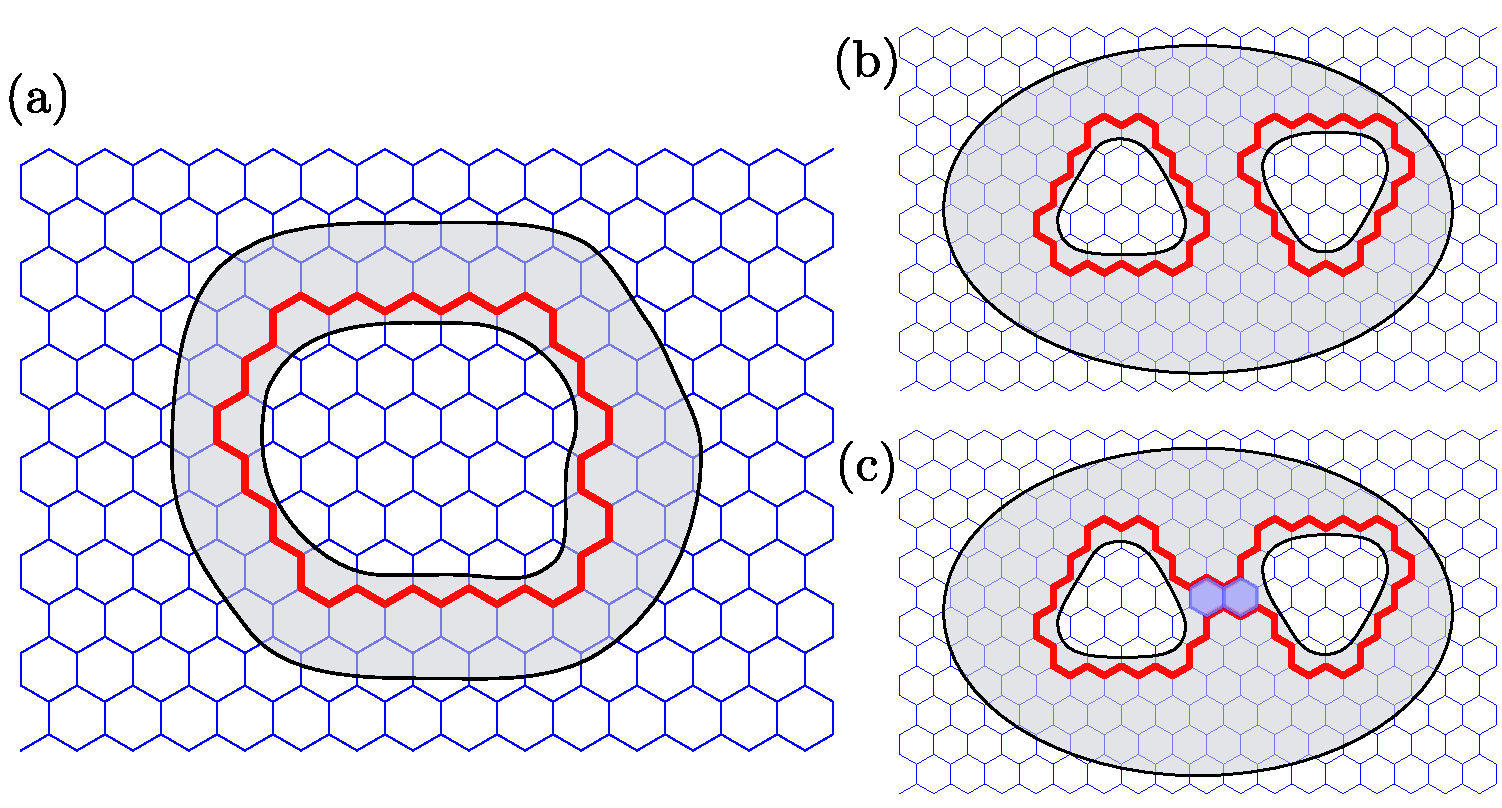
\includegraphics[width=\linewidth]{figures/non-contractable-loop-Group.pdf}
    \caption{(a) The loop in red stands for $\mathfrak{C}$, on which the operator $\Xi$ is defined. The loop is non-contractable in the shaded region $A$. Therefore, it plays a role as a non-contractable Wilson loop that gives rise to a topological term in the entanglement entropy. Operator $\Xi$ can be constructed by plaquette operators in a way described by equation \eqref{equ.Xi}, as the product of all plaquette operators inside or on the boundary of the inner hollow region. (b) If there is more than one hole in the region $A$, we can define different operators $\Xi^{(n)}$ corresponding to the $n$-th hole. (c) Two or more non-contractable loops circling different holes can merge into a larger loop circling those holes by acting plaquette operators to sew them together, as illustrated by the two blue plaquettes in the figure. Therefore, a large loop circling more than one hole does not count as an independent loop, because it can be built by combining individual loops together. This is one of the features of the $\mathbb{Z}_2$ theory.}
    \label{fig.non-contractable-loop}
\end{figure}

\begin{equation}\label{equ.Xi}
\Xi  = \frac{1}{2^{N^{\overline{A}}}}\Tr_{\overline{A}}\lr{\prod_{p\in\mrm{inner}}W_p} 
\end{equation}

\[\Xi  = \prod_{\anglelr{ij}\in\mathcal{C}_{\mrm{in}}\subset A}\sigma^{\alpha_{ij}}_i\sigma_j^{\alpha_{ij}} 
\]


\begin{equation}\label{equ.red-den-mat-not-sim-con}
    \rho_A = \frac{1}{2^{N^A-N_p^A-2}}\lr{\frac{\mathds{1}+\Xi}{2}}\mathcal{P}^{(p)}_A\sum_{[\mathfrak{D}]\subset A}\mathfrak{C}_{\mathfrak{D}}\Sigma_{\mathfrak{D}}
\end{equation}

The operator $\Xi$ describes a non-contractable loop $\mathfrak{C}$ in the subregion $A$ in the sense that there is no way to apply local operators $W_p$ to make $\mathfrak{C}$ shrink to a point in $A$. As shown in equation \eqref{equ.Xi}, the operator $\Xi$ depends on the chosen non-contractable loop $\mathfrak{C}\subset A$ and thus is not unique. However, the reduced density matrix $\rho_A$ is still uniquely given by equation \eqref{equ.red-den-mat-not-sim-con} because the projector $\mathcal{P}^{(p)}_A$ provides local operators $W_p$'s that relate different loops that are homeomorphic to $\mathfrak{C}$. More precisely, if two loops $\mathfrak{C}$ and $\mathfrak{C}'$ are homeomorphic, then we have
\[
\mathcal{P}^{(p)}_A\prod_{\anglelr{ij}\in\mathfrak{C}\subset A}\sigma^{\alpha_{ij}}_i\sigma^{\alpha_{ij}}_j = \mathcal{P}^{(p)}_A\prod_{\anglelr{ij}\in\mathfrak{C}'\subset A}\sigma^{\alpha_{ij}}_i\sigma^{\alpha_{ij}}_j
\]
Therefore, equation \eqref{equ.red-den-mat-not-sim-con} always gives a unique reduced density matrix even though the non-contractable loop $\mathfrak{C}$ is not unique.

\begin{equation}\label{equ.red-den-mat-general-g}
    \rho_A = \frac{1}{2^{N^A-N_p^A-2g}}\prod_{n=1}^{g}\lr{\frac{\mathds{1}+\Xi^{(n)}}{2}}\mathcal{P}^{(p)}_A\sum_{[\mathfrak{D}]\subset A}\mathfrak{C}_{\mathfrak{D}}\Sigma_{\mathfrak{D}}
\end{equation}

\alert{dimension of the density matrix is $2^{N^A-N^A_p-g}$}

}

\valert{
\subsection{Multiply Connected Regions}
\begin{equation}\label{equ.red-DM-new}
    \rho_A = \frac{1}{2^{N^A-N^A_p-2g}}\prod_{n=1}^{g}\lr{\frac{\mathds{1}+\Xi^{(n)}}{2}}\sum_{[\mathfrak{D}]\in A}\mathfrak{C}_{\mathfrak{D}}\mathcal{S}_\mathfrak{D}
\end{equation}
\[
    \rho_A^{F} = \frac{1}{2^{\lceil N^A/2 \rceil}}\sum_{[\mathfrak{D}]\in A}\mathfrak{C}_{\mathfrak{D}}\mathcal{M}_\mathfrak{D}
\]
There is no need to add the projector $\prod_{n=1}^{g}(\frac{\mathds{1}+\Xi^{(n)}}{2})$ in $\rho^{F}_A$, because the Majorana representation of the operator $\Xi$ is nothing more than identity
\[
\Xi^{(n)} = \prod_{\anglelr{ij}\in\mathcal{C}^{(n)}}ic_ic_j=\mathds{1}
\]
One can understand this fact in the sense that the topological property is completely encoded in the gauge sector.
\[
\rho^{FS}_A \equiv \frac{1}{2^{\lceil N^A/2 \rceil}} 
\prod_{n=1}^{g}\lr{\frac{\mathds{1}+\Xi^{(n)}}{2}}
\sum_{[\mathfrak{D}]\in A}\mathfrak{C}_{\mathfrak{D}}\mathcal{S}_\mathfrak{D}
\]
\[
\mathcal{S}^{(g)} \equiv \prod_{n=1}^{g}\lr{\frac{\mathds{1}+\Xi^{(n)}}{2}}\mathcal{P}_A^{(p)}\Sigma_{\mathfrak{D}}
\]
\[
\rho^{FS}_A \equiv \frac{1}{2^{\lceil N^A/2 \rceil}} 
\sum_{[\mathfrak{D}]\in A}\mathfrak{C}_{\mathfrak{D}}\mathcal{S}_\mathfrak{D}^{(g)}
\]
\[
\Tr \mathcal{S}_\varnothing^{(g)} = 2^{N^A-N^A_p-2g} = 2^{\lfloor N^A/2\rfloor-N^A_p-g}\Tr_F \mathcal{M}_\varnothing
\]
\[
\rho_A = \frac{1}{2^{\lfloor N^A/2\rfloor  -N^A_p - 2g}} \rho^{FS}_A
\]

If the region is not simply connected and hence has a non-zero genus number $g$, then formula \eqref{equ.Pick_sim-con} can be generalized as follows:
\begin{equation}\label{equ.Pick_gen-con}
    \abs{\de A} = N^A - 2N^A_p + 2(1-g)
\end{equation}

\alert{conclude the origin of the topological entanglement entropy.}

\alert{$W_p$ equivalent class = gauge contribution. topological order arises from the glocal Wilson loop, since it provides the additional 1/2 factor, which can be generalized to the non-contractable loop caused by the region with a non-zero genus number. In summary, those projectors reduce the dimension, which makes an additional contribution of the entanglement entropy.}
}

\begin{figure}
    \centering
    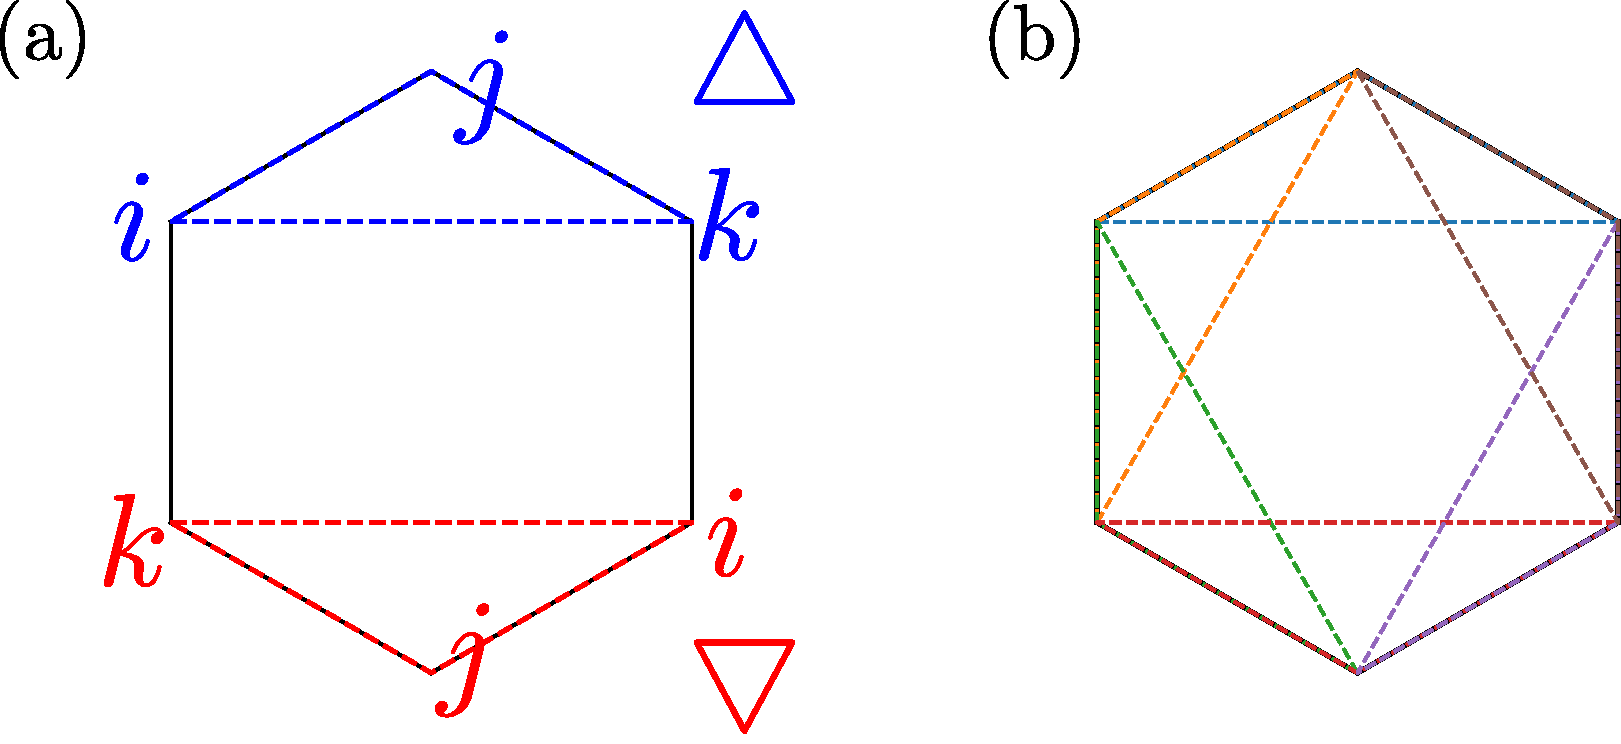
\includegraphics[width=0.7\linewidth]{figures/chiral-perturbation.pdf}
    \caption{(a) ~\cite{Xiang-3-spin-chiral} (b) A generalization of the previous perturbation proposed by Ref.~\cite{Xiang-3-spin-chiral} that preserves the $C_3$ point symmetry of the honeycomb lattice. Each triangle at the corner $j$ of the hexagon stands for $\sigma_i^{\mu_i}\sigma_j^{\mu_j}\sigma_k^{\mu_k}$~\cite{3-spin-1, 3-spin-2, 3-spin-3, 3-spin-4}. \alert{more}}
    \label{fig.up-down-triangle}
\end{figure} 

%%%%%%%%%%%%%%%%%%%%

We observed that the order of the product becomes important once the endpoints of the string are in the same sublattice. See Fig.~\ref{fig.standard-configuration} for example. The string $\mathfrak{D}_1$ has two endpoints, one of which belongs to the sublattice $A$, marked by a black dot, and the other belongs to $B$, marked by a hollow circle. Such a string consists of seven edges, and the corresponding string operator can be defined in such a way that the order of the product is from the type-$A$ endpoint to the type-$B$ endpoint: 
\[
\Sigma_{\mathfrak{D}_1} = \lr{12}\lr{23}\lr{34}\lr{45}\lr{56}\lr{67}\lr{78}
\]
where we denoted by $\lr{ij}\equiv\dimer{i}{j}$ the string operator of a single edge connecting adjacent sites $i$ and $j$ along $\mathfrak{D}_1$, and the lattice site 1 is in sublattice $A$ as illustrated in Fig.~\ref{fig.standard-configuration}. We find another definition in reverse order 
\[
\Sigma_{\mathfrak{D}_1}' = \lr{87}\lr{76}\lr{65}\lr{54}\lr{43}\lr{32}\lr{21}
\]
is equal to the previous definition: $\Sigma_{M_1}=\Sigma_{\mathfrak{D}_1}'$. On the other hand, consider the string operator corresponding to $\mathfrak{D}_2$ containing four edges, its definition could be
\[
\Sigma_{\mathfrak{D}_2} = \lr{12}\lr{23}\lr{34}\lr{45}
\]
where lattice site 1 is the endpoint of the string on the left-hand side, while another definition is
\[
\Sigma_{\mathfrak{D}_2}'=\lr{54}\lr{43}\lr{32}\lr{21}
\]
is different from $\Sigma_{\mathfrak{D}_2}$ by a sign: $\Sigma_{\mathfrak{D}_2}=-\Sigma_{\mathfrak{D}_2}'$. From these two examples, we find that the string operator of a single string with two endpoints in the different sublattices has a unique definition, whereas the one with two endpoints in the same sublattice does not. In all, 

%%%%%%%%%%%%%%%%%%%%%%%%%%%%%

\alert{The benefit of using the Majorana representation}

\alert{Although Ref.~\cite{Yao-Qi} has already given the formula to calculate the entanglement entropy of the Kitaev model, there are still some problems and remaining questions to ask. First of all, the method used in Ref.~\cite{Yao-Qi} is valid only for chosen subregions $A$ having an even number of lattice sites, that is, $N^A$ must be even. However, there is no reason to impose such a restriction, and so the result should hold based on a more general setting. Second, Ref.~\cite{Yao-Qi} used the replica trick~\cite{Callan-Wilczek, Holzhey-Larsen-Wilczek-CFT, Calabrese-Cardy-CFT_1, Calabrese-Cardy-CFT_2} to compute the entanglement entropy. Although most of the time the replica trick gives the correct value of the entanglement entropy, the mathematical background about such an analytical continuation is still not rigorous enough. The last question we would like to address is, Ref.~\cite{Yao-Qi} only gave the derivation of the entanglement entropy; therefore, the direct analysis of the entanglement spectrum is still lacking. The result of the entanglement entropy can only imply the structure of the entanglement spectrum, but cannot be used as the source of the full information about it. }

%%%%%%%%%%%%%%%%%%%%%%%%%%%%%%%

\alert{Now we discuss the density matrix of the ground state of the Kitaev model.  As pointed out by equation \eqref{equ.only-finite-correlation}, finite spin-correlation functions of the Kitaev ground state must be of the following form
\[
\anglelr{\prod_{\anglelr{ij}\in \mathfrak{D}}\sigma^{\alpha_{ij}}_i\sigma^{\alpha_{ij}}_j} = \anglelr{\Sigma_{\mathfrak{D}}}
\]
Otherwise, the correlation function vanishes. That means, in the expansion \eqref{equ.rho-starting}, we only have to consider correlation functions of the form $\anglelr{\Sigma_{\mathfrak{D}}}$. Thus, it seems that the density matrix is of the form 
\[
\rho = \frac{1}{2^N}\sum_{\mathfrak{D}}\mathfrak{C}_\mathfrak{D}\Sigma_\mathfrak{D}
\]
where we have denoted by $\mathfrak{C}_\mathfrak{D}$ the expectation value of the string operator $\anglelr{\Sigma_\mathfrak{D}}$. However, as we have observed, the string operators $\Sigma_{\mathfrak{D}\oplus\mathfrak{D}_Z}$ and $\Sigma_{\mathfrak{D}\oplus\mathfrak{D}_{zz}}$ for an arbitrary $\mathfrak{D}$ are completely identical, and so they shall not be included in the density matrix at the same time. Otherwise, it will lead to double-counting. Nevertheless, it is still more convenient to include all the configurations than to exclude $\mathfrak{D}_{zz}$ from the density matrix. Therefore, to prevent double-counting, we directly divide the previous form of the density matrix by two 
\begin{equation}\label{equ.rho-Sigma}
    \rho = \frac{1}{2^{N+1}}\sum_{\mathfrak{D}}\mathfrak{C}_\mathfrak{D}\Sigma_\mathfrak{D}
\end{equation}
Only then is this the correct density matrix.
 
According to the physical picture of equivalence class given by equation \eqref{equ.string-operator-equivalent}, the summation in \eqref{equ.rho-Sigma} can be sorted into different classes
\[
\sum_{\mathfrak{D}}\mathfrak{C}_{\mathfrak{D}}\Sigma_\mathfrak{D} = \sum_{[\mathfrak{D}^c]}\sum_{\mathfrak{D}\in[\mathfrak{D}^c]}\mathfrak{C}_{\mathfrak{D}}\Sigma_\mathfrak{D}
\]
By definition, an equivalence class $[\mathfrak{D}^c]$ consists of edge configurations that can be related to $\mathfrak{D}^c$ by combining with local or global loops. Therefore, summing over edge configurations in an equivalence class can be rewritten as summing over all loops combined with the character $\mathfrak{D}^c$
\begin{align}\label{equ.class-rep-by-loops}
    &\sum_{\mathfrak{D}\in[\mathfrak{D}^c]}\mathfrak{C}_\mathfrak{D}\Sigma_\mathfrak{D}  \nonumber\\
    =& \lr{\mathds{1}+\Tilde{W}_h}\lr{\mathds{1}+\Tilde{W}_v}\lr{\sum_{\mathcal{A}}'\prod_{p\in\mathcal{A}}W_p} \mathfrak{C}_{\mathfrak{D}^c}\Sigma_{\mathfrak{D}^c}.
\end{align}
with $\mathcal{A}$ denoting different sets of plaqette configurations defined in \eqref{equ.lattice-Stokes}. We point out that, due to the identity $\prod_{p}W_p=\mathds{1}$, the loop constructed by $\prod_{p\in \mathcal{A}}W_p$ is identical to that constructed by $\prod_{p\in \overline{\mathcal{A}}}W_p$ with $\overline{\mathcal{A}}$ representing the complement of $\mathcal{A}$. Therefore, we only have to sum over distinct loops, and the primed summation in \eqref{equ.class-rep-by-loops} precisely stands for such a summation. In other words, the plaquette configurations included in the summation are those with size smaller than half of the entire system. It turns out that the summation can be factorized thanks to the following identity
\begin{align}
    \prod_{p}\lr{\mathds{1}+W_p} &= \lr{\mathds{1}+\prod_{p}W_p}\sum'_{\mathcal{A}}\prod_{p\in\mathcal{A}}W_p \nonumber\\
    &= 2\sum'_{\mathcal{A}}\prod_{p\in\mathcal{A}}W_p.
\end{align}
Substituting \eqref{equ.W-prod-expansion} into \eqref{equ.class-rep-by-loops} and then plugging the result into \eqref{equ.class-sum} gives the following form of the density matrix
\begin{equation}\label{equ.factorize}
\rho = \sum_{[\mathfrak{D}^c]}\mathfrak{C}_{\mathfrak{D}^c}
\frac{1}{4} \lrm{\lr{\mathds{1}+\Tilde{W}_h}\lr{\mathds{1}+\Tilde{W}_v}\prod_p\lr{\mathds{1}+W_p}}\Sigma_{\mathfrak{D}^c}
\end{equation}
in which we can see that the projector \eqref{equ.p-projector} appears. With proper coefficients, we ultimately obtain the density matrix of the Kitaev ground state

where we denoted by $\mathcal{P}_{\mrm{topo}}$ the projector onto the subspace with fixed eigenvalues of the two global Wilson loops $\Tilde{W}_h$ and $\Tilde{W}_v$, 
\[
\mathcal{P}_{\mrm{topo}}\equiv \lr{\frac{\mathds{1}+\Tilde{W}_h}{2}}\lr{\frac{\mathds{1}+\Tilde{W}_v}{2}}
\]
} 